% ===========================================================================
% RELATORIO — Roteiro 3, Amplificador Operacional: Nao-idealidades
% ENE0046 Laboratorio de Eletronica 2026/2 — Equipe 1, Turma 04
% ===========================================================================
\documentclass[11pt,a4paper]{article}
\input{estilo-relatorio}
\usepackage{float} % figuras [H]: ficam exatamente onde estão no texto, sem flutuar

% --------------------------- IDENTIFICACAO ---------------------------------
\roteiro{3}{Amplificador Operacional: Não-idealidades}
\aturma{04}

\autorum{Ana Luísa Reis Nascente}{211045688}
\autordois{Gabriel de Sousa}{211056000}
% ---------------------------------------------------------------------------

\begin{document}
\capa

\begin{resumo}
Este relatório caracteriza tensão de offset, corrente de polarização, resposta em frequência
e slew rate em amplificadores operacionais, por simulação individual e ensaios de bancada.
As medições indicaram offsets de \(0{,}156\) e \(0{,}167\,\text{mV}\) nos dois LM741,
e correntes de entrada de aproximadamente \(50{,}3\,\text{nA}\) no LM741 e
\(16{,}5\,\text{pA}\) no TL064. A simulação com os resistores medidos forneceu cortes de
\(96{,}00\) e \(10{,}20\,\text{kHz}\) para os estágios de ganhos nominais 11 e 101.
Na bancada, o estágio de ganho baixo apresentou distorção por slew rate durante a varredura,
o que impede interpretar sua queda de amplitude como medida isolada da largura de banda.
Para o ganho alto, um ajuste de um polo aos pontos completos forneceu corte estimado de
\(15{,}50\,\text{kHz}\), acima do simulado. Os slew rates medidos foram
\(0{,}314\) e \(3{,}442\,\text{V}/\mu\text{s}\), indicando resposta aproximadamente
onze vezes mais rápida do TL064. As comparações distinguem efeitos dos resistores,
limitações dos modelos e limitações do procedimento experimental.

\end{resumo}

\section{Introdução}

O modelo do amplificador operacional ideal — ganho infinito, entradas que não drenam corrente,
saída que responde instantaneamente e sem limite — é ferramenta poderosa para projetar um
circuito, mas nenhuma dessas quatro promessas se sustenta num dispositivo real. O par
diferencial de entrada nunca é perfeitamente simétrico, e essa assimetria aparece como uma
tensão de offset que qualquer estágio de ganho amplifica junto com o sinal — é o motivo pelo
qual um amplificador de instrumentação de alta precisão anuncia, no datasheet, um \(V_{os}\)
máximo em microvolts, não em zero. As mesmas entradas, para polarizar os transistores internos,
drenam uma corrente contínua pequena mas não nula; sobre a resistência de uma fonte de sinal de
alta impedância, essa corrente produz uma tensão de erro que compete com o próprio sinal, e é
por isso que um sensor de alta impedância prefere um amplificador de entrada JFET ou MOSFET a um
de entrada bipolar. O ganho de malha aberta, por sua vez, não é plano: cai com a frequência como
um passa-baixas de primeira ordem, e é essa queda, multiplicada pelo ganho fechado do estágio,
que limita a banda passante de qualquer amplificador realimentado — o mesmo produto ganho por
banda que aparece na folha de dados de qualquer AmpOp de uso geral. Por fim, o estágio de saída
não consegue variar tensão mais rápido que uma taxa máxima, o slew rate: acima de uma certa
combinação de amplitude e frequência, mesmo um sinal de entrada perfeitamente senoidal sai como
um triângulo — uma distorção não linear, diferente da atenuação linear da largura de banda, e
responsável por boa parte da distorção de sinais de áudio e vídeo de grande excursão em
amplificadores mal especificados.

Este roteiro mede as quatro não-idealidades no LM741 e compara corrente de
polarização e slew rate com o TL064, de entrada JFET. A comparação evidencia a menor
corrente de entrada e a maior taxa de variação de saída observadas no TL064. A etapa de simulação usa uma especificação numérica derivada da matrícula de cada
integrante (os ganhos \(G_1\) e \(G_2\) da resposta em frequência e a amplitude \(V_p\) do slew
rate), de modo que cada um projeta seu próprio par de resistores em série E12; a etapa de
bancada usa uma segunda especificação, definida pelo número da equipe, e é montada uma única vez
pela equipe inteira.

O restante deste relatório está organizado como segue: a Seção~\ref{sec:teoria} deduz as quatro
expressões usadas para extrair \(V_{os}\), \(I_b\), a frequência de corte e o slew rate a partir
das medidas brutas; a Seção~\ref{sec:espec} aplica essas expressões à especificação da matrícula
de Ana e escolhe os resistores comerciais da resposta em frequência; o projeto de Gabriel
é detalhado na Seção~\ref{sec:gabriel-simulacoes}; a Seção~\ref{sec:metodo}
descreve cada simulação e a montagem em bancada; a Seção~\ref{sec:resultados} traz os resultados
numéricos de projeto, simulação e medição; a Seção~\ref{sec:discussao} discute as divergências
entre essas três etapas; e a Seção~\ref{sec:conclusao} fecha com as conclusões.

\section{Fundamentação teórica}
\label{sec:teoria}

\subsection{Amplificador não inversor: o circuito comum às quatro medidas}

As quatro não-idealidades deste roteiro são medidas sobre a mesma topologia base: um amplificador
não inversor, com a entrada não inversora recebendo o sinal (ou o terra, ou um resistor ao
terra) e a realimentação fixada por \(R_f\) (da saída ao nó inversor) e \(R_g\) (do nó inversor
ao terra). Com o AmpOp em realimentação negativa e ganho de malha aberta \(A_v\) muito maior que
o ganho fechado pretendido, as duas entradas ficam praticamente no mesmo potencial (curto
virtual). Chamando de \(v_i\) o potencial da entrada não inversora, o nó inversor também fica em
\(v_i\), e a corrente que entra por \(R_g\) é a mesma que sai por \(R_f\), já que a entrada do
AmpOp não drena corrente:

\begin{equation}
\frac{v_i}{R_g} = \frac{v_o - v_i}{R_f} \quad\Rightarrow\quad
G = \frac{v_o}{v_i} = 1 + \frac{R_f}{R_g}
\label{eq:naoinversor}
\end{equation}

Essa mesma relação, aplicada a diferentes "entradas efetivas" \(v_i\), é a base das duas
primeiras não-idealidades. Vale registrar por que o curto virtual se sustenta: se, por qualquer
perturbação, \(V_-\) se afastasse de \(V_+\), o ganho de malha aberta \(A_v\) (tipicamente
\(10^5\)–\(10^6\)) amplificaria essa diferença por um fator enorme na saída; como a saída
realimenta o próprio nó inversor por \(R_f\), esse desvio na saída empurra \(V_-\) de volta na
direção de \(V_+\) até a diferença ficar desprezível. É esse mecanismo — e não uma propriedade
"mágica" do AmpOp — que faz o curto virtual valer na prática, e é também ele que, mais adiante
(Seção~\ref{sec:teoria-freq}), deixa de funcionar bem quando \(A_v\) cai com a frequência: sem
ganho de malha aberta suficiente, o erro entre \(V_+\) e \(V_-\) deixa de ser desprezível, e o
ganho fechado começa a cair.

\subsection{Tensão de offset}

Com a entrada não inversora ligada diretamente ao terra, um AmpOp ideal daria \(v_o=0\). O AmpOp
real, porém, tem uma assimetria interna no par diferencial de entrada, equivalente a uma fonte
contínua \(V_{os}\) em série com uma das entradas — fisicamente, \(V_{os}\) ocupa o lugar de
\(v_i\) na Equação~\eqref{eq:naoinversor}, mesmo com a entrada externa aterrada:

\begin{equation}
V_o = V_{os}\left(1+\frac{R_f}{R_g}\right) \quad\Rightarrow\quad
V_{os} = \frac{V_o}{1+R_f/R_g}
\label{eq:offset}
\end{equation}

Com \(R_f=100\,\text{k}\Omega\) e \(R_g=1\,\text{k}\Omega\) (Seção~2.1 do roteiro), o ganho vale
\(101\), e a Equação~\eqref{eq:offset} se reduz a \(V_{os}=V_o/101\): a saída, embora pequena, é
o offset de entrada amplificado cem vezes, o que a torna mensurável com um multímetro comum.

Fisicamente, \(V_{os}\) vem do par diferencial de entrada do AmpOp — dois transistores que, no
projeto ideal, seriam idênticos, mas que saem da fabricação com uma pequena diferença de área de
emissor, de dopagem ou de tensão de limiar entre si. Essa assimetria faz um dos dois transistores
conduzir um pouco mais que o outro mesmo com as duas bases (ou portas) no mesmo potencial, e a
única forma de zerar essa diferença de corrente é aplicar entre as entradas uma pequena tensão
externa — é essa tensão, entre poucos microvolts e poucos milivolts, que o modelo representa como
\(V_{os}\). Por ser um efeito de descasamento aleatório de fabricação, \(V_{os}\) varia de
exemplar para exemplar do mesmo modelo (o que a troca de LM741 na Seção~3.3 evidencia
diretamente), tem sinal imprevisível a priori, e não é algo que aumentar a alimentação ou mudar o
ganho resolva — só uma malha de ajuste (trim) ou uma topologia diferencial melhor casada reduz
seu efeito.

\subsection{Corrente de polarização}

As entradas de um AmpOp real drenam uma corrente contínua \(I_b\) para polarizar o par
diferencial interno. Inserindo um resistor \(R_s\) entre o terra e a entrada não inversora
(Seção~2.2), essa corrente passa a produzir, sobre \(R_s\), uma tensão \(I_b R_s\) que se soma ao
\(V_{os}\) já presente — o novo "\(v_i\)" efetivo da Equação~\eqref{eq:naoinversor} é
\(V_{os}+I_bR_s\):

\begin{equation}
V_o' = \left(V_{os}+I_bR_s\right)\left(1+\frac{R_f}{R_g}\right)
\label{eq:bias-vo}
\end{equation}

Subtraindo a Equação~\eqref{eq:offset} (o mesmo circuito, sem \(R_s\)) da Equação~\eqref{eq:bias-vo}
— o termo de \(V_{os}\) é comum aos dois circuitos e se cancela —, chega-se à expressão que o
roteiro pede:

\begin{equation}
\Delta V_o = V_o' - V_o = I_b R_s\left(1+\frac{R_f}{R_g}\right)
\quad\Rightarrow\quad
I_b = \frac{\Delta V_o}{101\, R_s}
\label{eq:bias}
\end{equation}

O sinal de \(I_b\) obtido por essa conta indica o sentido físico da corrente: um valor negativo
(a saída \emph{cai} quando \(R_s\) entra) diz que a corrente na verdade entra no pino, drenada da
malha externa — o que se espera de um par de entrada bipolar NPN, que precisa de corrente de
base fornecida pelo circuito externo.

A origem física de \(I_b\) explica também por que ela muda tanto de uma tecnologia de entrada
para outra. No LM741, a entrada é o par diferencial bipolar propriamente dito: cada transistor
precisa de uma corrente de base \(I_b=I_c/\beta\) para sustentar a corrente de coletor que o
polariza, e com \(\beta\) tipicamente na faixa de \(100\)–\(300\) e correntes de coletor de
polarização na casa de microampères, \(I_b\) cai naturalmente na faixa de dezenas a centenas de
nanoampères — e, por ser corrente de base de um transistor NPN, só pode fluir para dentro do
pino, nunca para fora, explicando por que a saída caiu (e não subiu) nas duas peças testadas. Já
no TL064, a entrada é a porta de um JFET: não existe corrente de base nesse sentido, e o que
flui pelo pino é só a corrente de fuga reversa da junção porta-canal, ordens de grandeza menor
(tipicamente picoampères) porque uma junção reversamente polarizada conduz muito pouco em
comparação com a corrente direta de base de um bipolar. É essa diferença de mecanismo — corrente
de base contra corrente de fuga de junção — que está por trás da razão de milhares de vezes
observada entre as duas peças, não apenas uma diferença de grau dentro da mesma tecnologia.

\subsection{Resposta em frequência}
\label{sec:teoria-freq}

O ganho de malha aberta \(A_v(jf)\) de um AmpOp de uso geral cai com a frequência como um
passa-baixas de primeiro polo, \(A_v(jf)=A_{v0}/(1+jf/f_b)\), com \(A_{v0}\) enorme e \(f_b\)
baixíssimo (poucos hertz). O produto desses dois números — o produto ganho por banda,
\(\text{GBW}=A_{v0}f_b\) — é a frequência em que o ganho de malha aberta cruzaria a unidade, e é
uma característica fixa do dispositivo, independente do ganho fechado escolhido. Substituindo
\(A_v(jf)\) na malha fechada (ganho ideal \(G=1+R_f/R_g\), realimentação \(\beta=1/G\)) e usando
\(A_{v0}\beta\gg1\), o ganho fechado também se comporta como um passa-baixas de primeiro polo:

\begin{equation}
A_{cl}(jf) \approx \frac{G}{1+jf/f_c}, \qquad f_c = \frac{\text{GBW}}{G}
\label{eq:corte}
\end{equation}

Ou seja, a frequência de corte de malha fechada (onde o ganho cai a \(0{,}707\) do valor em baixa
frequência, \(-3\,\text{dB}\)) é o produto ganho por banda dividido pelo ganho fechado — e por
isso o produto \(G\cdot f_c\), medido de volta a partir do corte observado, deve dar
aproximadamente o mesmo número (o GBW do dispositivo) não importa qual dos dois ganhos do
roteiro (\(G_1\) ou \(G_2\)) seja usado para medi-lo.

O motivo de existir um único polo dominante tão baixo (poucos hertz) não é acidental: um AmpOp de
uso geral como o LM741 é construído com um capacitor de compensação interno (da ordem de
\(30\,\text{pF}\) no caso do LM741), colocado deliberadamente entre um dos estágios internos de
ganho, exatamente para criar esse polo dominante bem abaixo de qualquer outro polo parasita do
circuito. Sem essa compensação, os vários estágios internos de ganho contribuiriam cada um com
seu próprio polo em frequências relativamente próximas, e a soma das suas defasagens ultrapassaria
\(180^\circ\) ainda com ganho de malha maior que \(1\) quando o AmpOp fosse realimentado com ganho
unitário — a condição clássica de instabilidade, que faria o circuito oscilar em vez de amplificar.
O capacitor de compensação sacrifica banda passante (empurra o primeiro polo para uma frequência
muito baixa) em troca de garantir que o ganho de malha aberta já caiu abaixo da unidade bem antes
de qualquer polo parasita atrasar o sinal o suficiente para instabilizar o circuito — é a mesma
lógica de projeto por trás de todo AmpOp "unity-gain stable" de uso geral.

\subsection{Slew rate}

O slew rate é o limite físico de quão rápido a tensão de saída do AmpOp pode variar,
normalmente expresso em \(\text{V}/\mu\text{s}\). Uma senoide de amplitude \(V_p\) e frequência
\(f\), \(v_o(t)=V_p\sin(2\pi ft)\), tem sua maior taxa de variação exatamente na passagem por
zero:

\begin{equation}
\left.\frac{dv_o}{dt}\right|_{\max} = 2\pi f V_p
\label{eq:slew-taxa}
\end{equation}

Enquanto essa taxa fica abaixo do slew rate do dispositivo, a saída acompanha a entrada
fielmente. Quando a Equação~\eqref{eq:slew-taxa} ultrapassa o \(SR\) do AmpOp, o estágio de saída
não consegue mais seguir a senoide: ele sobe e desce à taxa máxima constante \(SR\), e a forma de
onda observada deixa de ser senoidal e passa a ser um triângulo, cujo pico já não atinge mais
\(V_p\). Igualando a Equação~\eqref{eq:slew-taxa} a \(SR\), obtém-se a frequência limiar a partir
da qual esse efeito aparece:

\begin{equation}
f_{max} = \frac{SR}{2\pi V_p}
\label{eq:slew-fmax}
\end{equation}

Diferentemente do corte da Equação~\eqref{eq:corte}, esse limite depende da amplitude do sinal:
dobrar \(V_p\) reduz \(f_{max}\) à metade, mesmo com o mesmo \(SR\) — é por isso que a frequência
de corte medida na Seção~\ref{sec:teoria-freq} não é, em geral, o mesmo número que o limiar de
slew rate, e a Seção~3.5 do roteiro pede para identificar qual dos dois uma curva de resposta em
frequência encontra primeiro.

O slew rate tem origem no mesmo capacitor de compensação da Seção~\ref{sec:teoria-freq}: o
estágio de entrada do AmpOp só consegue fornecer uma corrente máxima \(I_{max}\) (limitada pela
própria corrente de polarização dos transistores de entrada) para carregar e descarregar esse
capacitor \(C_c\), e a tensão sobre um capacitor não pode variar mais rápido do que
\(dV/dt=I/C\). Quando a saída pede uma variação de tensão mais rápida do que
\(SR=I_{max}/C_c\) consegue entregar, o estágio de entrada satura tentando fornecer o máximo de
corrente que tem, o capacitor de compensação carrega à taxa constante \(I_{max}/C_c\) em vez de
seguir a forma de onda pedida, e é exatamente esse carregamento à taxa constante que aparece como
o segmento reto da rampa triangular observada. O produto ganho por banda e o slew rate, embora dependam de parâmetros internos do amplificador,
são especificações diferentes: o primeiro descreve a resposta linear de pequeno sinal;
o segundo limita a taxa de variação para sinais de maior amplitude. Uma tecnologia de
entrada, por si só, não determina uma relação universal entre essas grandezas.

\section{Especificação e projeto}
\label{sec:espec}

\begin{espec}
Matrícula \mat{211045688}, na forma ABCDEFGHI: A=2, B=1, C=1, D=0, EF=45, GH=68, I=8.
\begin{align*}
G_1 &= 20+(\text{EF}\bmod{21}) = 20+(45\bmod{21}) = 20+3 = 23 \\
G_2 &= 80+(\text{GH}\bmod{41}) = 80+(68\bmod{41}) = 80+27 = 107 \\
V_p &= 2+\text{I}/2 = 2+8/2 = 6\text{ V}
\end{align*}
\end{espec}

Resistores da série E12, entre \(1\,\text{k}\Omega\) e \(100\,\text{k}\Omega\), cada perna da
rede de realimentação com até dois resistores em série. Alimentação simétrica de
\(\pm15\,\text{V}\). As Seções~2.1 e 2.2 do roteiro (tensão de offset e corrente de polarização)
usam valores fixos, independentes da matrícula: \(R_f=100\,\text{k}\Omega\),
\(R_g=1\,\text{k}\Omega\) (ganho \(101\)) e \(R_s=100\,\text{k}\Omega\). Só a resposta em
frequência (Seção~2.3) exige projetar os resistores a partir de \(G_1\) e \(G_2\); o slew rate
(Seção~2.4) usa a mesma amplitude \(V_p\) da especificação, sem componente a dimensionar.

\subsection{Resposta em frequência: projeto dos dois ganhos}

De \eqref{eq:naoinversor}, \(R_f/R_g=G-1\): \(22\) para o estágio de ganho \(G_1=23\), e \(106\)
para o estágio de ganho \(G_2=107\). Testando combinações E12 (um resistor ou dois em série por
perna):

\begin{center}\small
\setlength{\tabcolsep}{4pt}
\begin{tabular}{@{}lrlrrr@{}}
\toprule
\textbf{Estágio} & \textbf{\(R_f/R_g\) necessário} & \textbf{Combinação E12} &
\textbf{\(R_f/R_g\) realizado} & \textbf{\(G\) realizado} & \textbf{Desvio} \\
\midrule
1 (\(G_1=23\)) & 22 & \(R_g{=}1\,\text{k}\Omega\), \(R_f{=}22\,\text{k}\Omega\) &
  \(22{,}000\) & \(23{,}000\) & \(0{,}00\%\) \\
2 (\(G_2=107\)) & 106 & \(R_g{=}1{,}2\,\text{k}\Omega\), \(R_f{=}100\,\text{k}\Omega{+}27\,\text{k}\Omega\) &
  \(105{,}833\) & \(106{,}833\) & \(-0{,}16\%\) \\
\bottomrule
\end{tabular}
\end{center}

O estágio 1 fechou exato porque \(22\,\text{k}\Omega/1\,\text{k}\Omega\) já é uma razão E12
direta. Para o estágio 2, uma alternativa (\(R_g{=}1\,\text{k}\Omega\),
\(R_f{=}100\,\text{k}\Omega{+}5{,}6\,\text{k}\Omega=105{,}6\,\text{k}\Omega\)) chegava a
\(-0{,}37\%\) de desvio; trocando \(R_g\) para \(1{,}2\,\text{k}\Omega\) e \(R_f\) para
\(100\,\text{k}\Omega{+}27\,\text{k}\Omega=127\,\text{k}\Omega\), o desvio caiu para
\(-0{,}16\%\), a melhor combinação testada dentro do limite de dois resistores em série por
perna.

\section{Metodologia}
\label{sec:metodo}

Cada AmpOp foi trazido ao LTspice como um símbolo de cinco terminais a partir do subcircuito em
\texttt{ene0046.lib}. Os símbolos reaproveitam os do Roteiro~2 e respeitam a ordem de
terminais de cada subcircuito; nos arquivos de Gabriel, chamam-se \texttt{LM741.asy} e \texttt{TL064.asy}. Cada
simulação usa alimentação \(\pm15\,\text{V}\) empilhada (duas fontes de \(15\,\text{V}\) com o
terra no nó do meio), a mesma técnica usada no Roteiro~2.

\subsection{Simulação de projeto, uma por integrante}

\subsubsection*{Ana Luísa Reis Nascente — matrícula 211045688}

Cada item foi simulado em arquivo próprio, de \texttt{item\_1.asc} a \texttt{item\_6.asc},
com uma análise por arquivo:

\begin{itemize}
\item \textbf{item\_1} — tensão de offset: não inversor de ganho \(101\) (\(R_f{=}100\,\text{k}\Omega\),
  \(R_g{=}1\,\text{k}\Omega\)) com a entrada não inversora aterrada por um fio próprio, em ponto
  de operação (\texttt{.op}).

  \begin{figure}[H]
\centering
\includegraphics[width=0.75\linewidth]{ana/item_1_circuito.png}
\caption{Esquemático do item\_1 (tensão de offset): não inversor de ganho \(101\) com o LM741,
entrada não inversora aterrada por um fio dedicado, sem tocar a malha de realimentação.}
\label{fig:item1}
\end{figure}

\item \textbf{item\_2} — corrente de polarização: mesmo circuito do item\_1, com
  \(R_s{=}100\,\text{k}\Omega\) entre o terra e a entrada não inversora, também em ponto de
  operação.

  \begin{figure}[H]
\centering
\includegraphics[width=0.75\linewidth]{ana/item_2_circuito.png}
\caption{Esquemático do item\_2 (corrente de polarização): o mesmo não inversor do item\_1, com
\(R_s{=}100\,\text{k}\Omega\) na entrada não inversora.}
\label{fig:item2}
\end{figure}

\item \textbf{item\_3} — resposta em frequência: os dois estágios não inversores
  (\(G_1{=}23\), \(G_2{=}107\)) no mesmo arquivo, alimentados pela mesma fonte AC, em varredura
  decádica (\texttt{.ac dec 50 10 10meg}). Um erro de montagem — o fio da entrada do segundo
  estágio reaproveitando o retorno da própria fonte \texttt{V3}, desligando-a do terra — chegou a
  acoplar os dois estágios entre si; corrigido com um fio e um \emph{net label} \texttt{Vin}
  independentes para a entrada do segundo estágio.

  \begin{figure}[H]
\centering
\includegraphics[width=0.85\linewidth]{ana/item_3_circuito.png}
\caption{Esquemático do item\_3 (resposta em frequência): dois não inversores independentes,
ganhos \(G_1{=}23\) e \(G_2{\approx}106{,}8\), compartilhando a fonte AC e a alimentação.}
\label{fig:item3}
\end{figure}

\item \textbf{item\_4} — slew rate: seguidor de tensão com o LM741, entrada senoidal de
  amplitude \(V_p{=}6\,\text{V}\), duas frequências por \texttt{.step} (\(5\,\text{kHz}\) e
  \(50\,\text{kHz}\)), escolhidas a partir do limiar de datasheet
  (\(f_{max}{\approx}13{,}26\,\text{kHz}\) para \(SR{=}0{,}5\,\text{V}/\mu\text{s}\)) com folga
  confortável dos dois lados.

  \begin{figure}[H]
\centering
\includegraphics[width=0.75\linewidth]{ana/item_4_circuito.png}
\caption{Esquemático do item\_4 (slew rate, LM741): seguidor de tensão, \texttt{.step} de
frequência entre \(5\,\text{kHz}\) e \(50\,\text{kHz}\).}
\label{fig:item4}
\end{figure}

\item \textbf{item\_5} — corrente de polarização com o TL064: mesmo circuito do item\_2,
  trocando o LM741 pelo TL064.

  \begin{figure}[H]
\centering
\includegraphics[width=0.75\linewidth]{ana/item_5_circuito.png}
\caption{Esquemático do item\_5 (corrente de polarização, TL064): mesmo circuito do item\_2 com
o TL064 no lugar do LM741.}
\label{fig:item5}
\end{figure}

\item \textbf{item\_6} — slew rate com o TL064: mesmo seguidor do item\_4, trocando o LM741 pelo
  TL064. As frequências do item\_4 não serviram (uma tentativa em \(200\,\text{kHz}\) só achatou a
  onda, sem triangular de forma clara); a segunda frequência foi refeita para
  \(500\,\text{kHz}\), mais de \(5\times\) o limiar de datasheet
  (\(f_{max}{\approx}92{,}9\,\text{kHz}\) para \(SR{=}3{,}5\,\text{V}/\mu\text{s}\)).

  \begin{figure}[H]
\centering
\includegraphics[width=0.75\linewidth]{ana/item_6_circuito.png}
\caption{Esquemático do item\_6 (slew rate, TL064): mesmo seguidor do item\_4 com o TL064,
\texttt{.step} de frequência entre \(5\,\text{kHz}\) e \(500\,\text{kHz}\).}
\label{fig:item6}
\end{figure}

\end{itemize}

\subsubsection*{Gabriel de Sousa — matrícula 211056000}

\label{sec:gabriel-simulacoes}

\begin{espec}
Matrícula \mat{211056000}: \(EF=56\), \(GH=00\to80\) e \(I=0\).
\begin{align*}
G_1 &= 20+(56\bmod21)=34, & G_2 &= 80+(80\bmod41)=119, & V_p &= 2+0/2=2\,\text{V}.
\end{align*}
\end{espec}

No item\_3, foram escolhidos \(R_{g1}=R_{g2}=1\,\text{k}\Omega\),
\(R_{f1}=33\,\text{k}\Omega\) e \(R_{f2}=100\,\text{k}\Omega+18\,\text{k}\Omega\).
Assim, \(G_1=1+33/1=34\) e \(G_2=1+(100+18)/1=119\), sem desvio nominal.
Todos são E12 e atendem à faixa de \(1\) a \(100\,\text{k}\Omega\) do Roteiro~3,
com no máximo dois resistores em série por perna. A alimentação é \(\pm15\,\text{V}\).

Os seis arquivos de Gabriel foram executados no LTspice XVII com a biblioteca
\texttt{ene0046.lib} fornecida. Foram conferidos os netlists, incluindo a ordem distinta
dos terminais dos dois modelos, e os esquemáticos na interface. As figuras seguintes
são capturas desses arquivos; os gráficos da Seção~\ref{sec:gabriel-resultados} foram
traçados a partir das amostras exportadas pelo simulador.

\paragraph{Item 1 — Tensão de offset} Não inversor com LM741, entrada não inversora aterrada, \(R_f=100\,\text{k}\Omega\), \(R_g=1\,\text{k}\Omega\) e análise \texttt{.op}.

\begin{figure}[H]
\centering
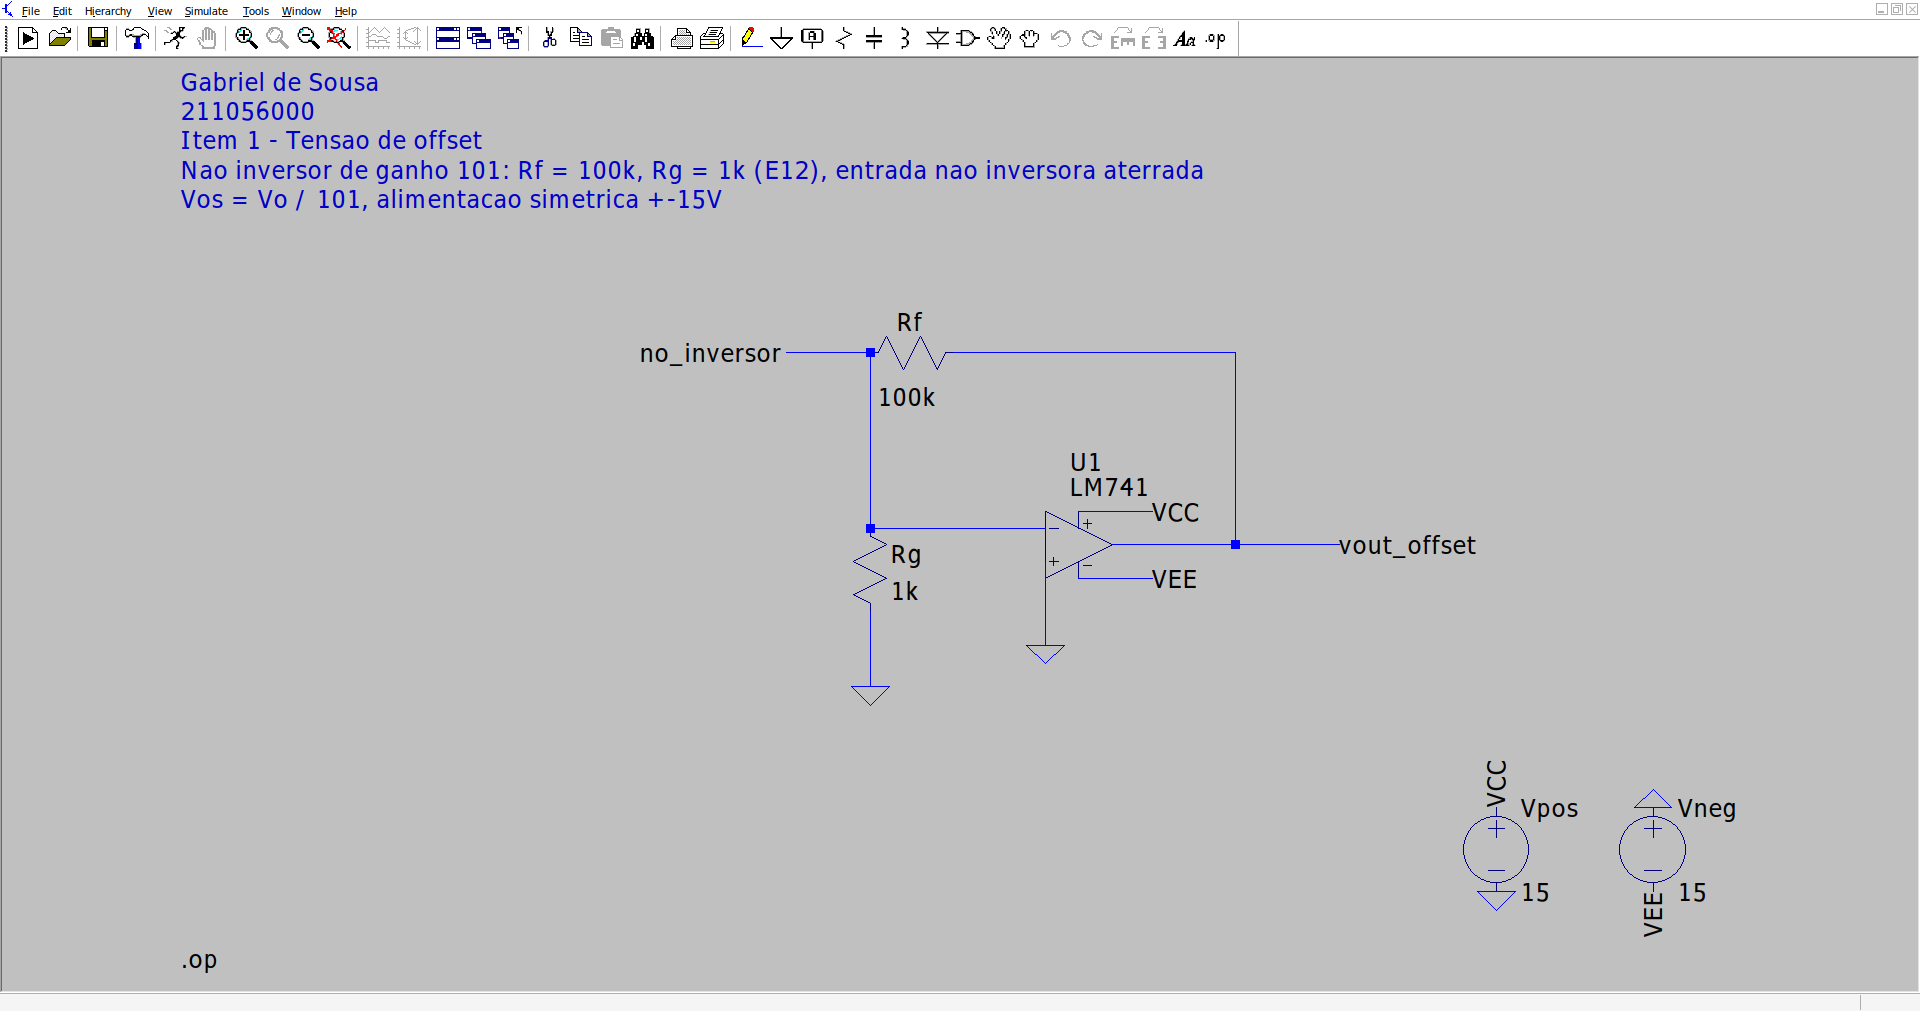
\includegraphics[width=\linewidth]{gabriel/item_1_circuito.png}
\caption{Gabriel, item\_1: circuito de ganho 101 para extração de \(V_{os}=V_o/101\).}
\label{fig:gabriel-item1}
\end{figure}

\paragraph{Item 2 — Corrente de polarização do LM741} Mesmo ganho do item\_1, acrescentando \(R_s=100\,\text{k}\Omega\) entre a entrada não inversora e o terra; análise \texttt{.op}.

\begin{figure}[H]
\centering
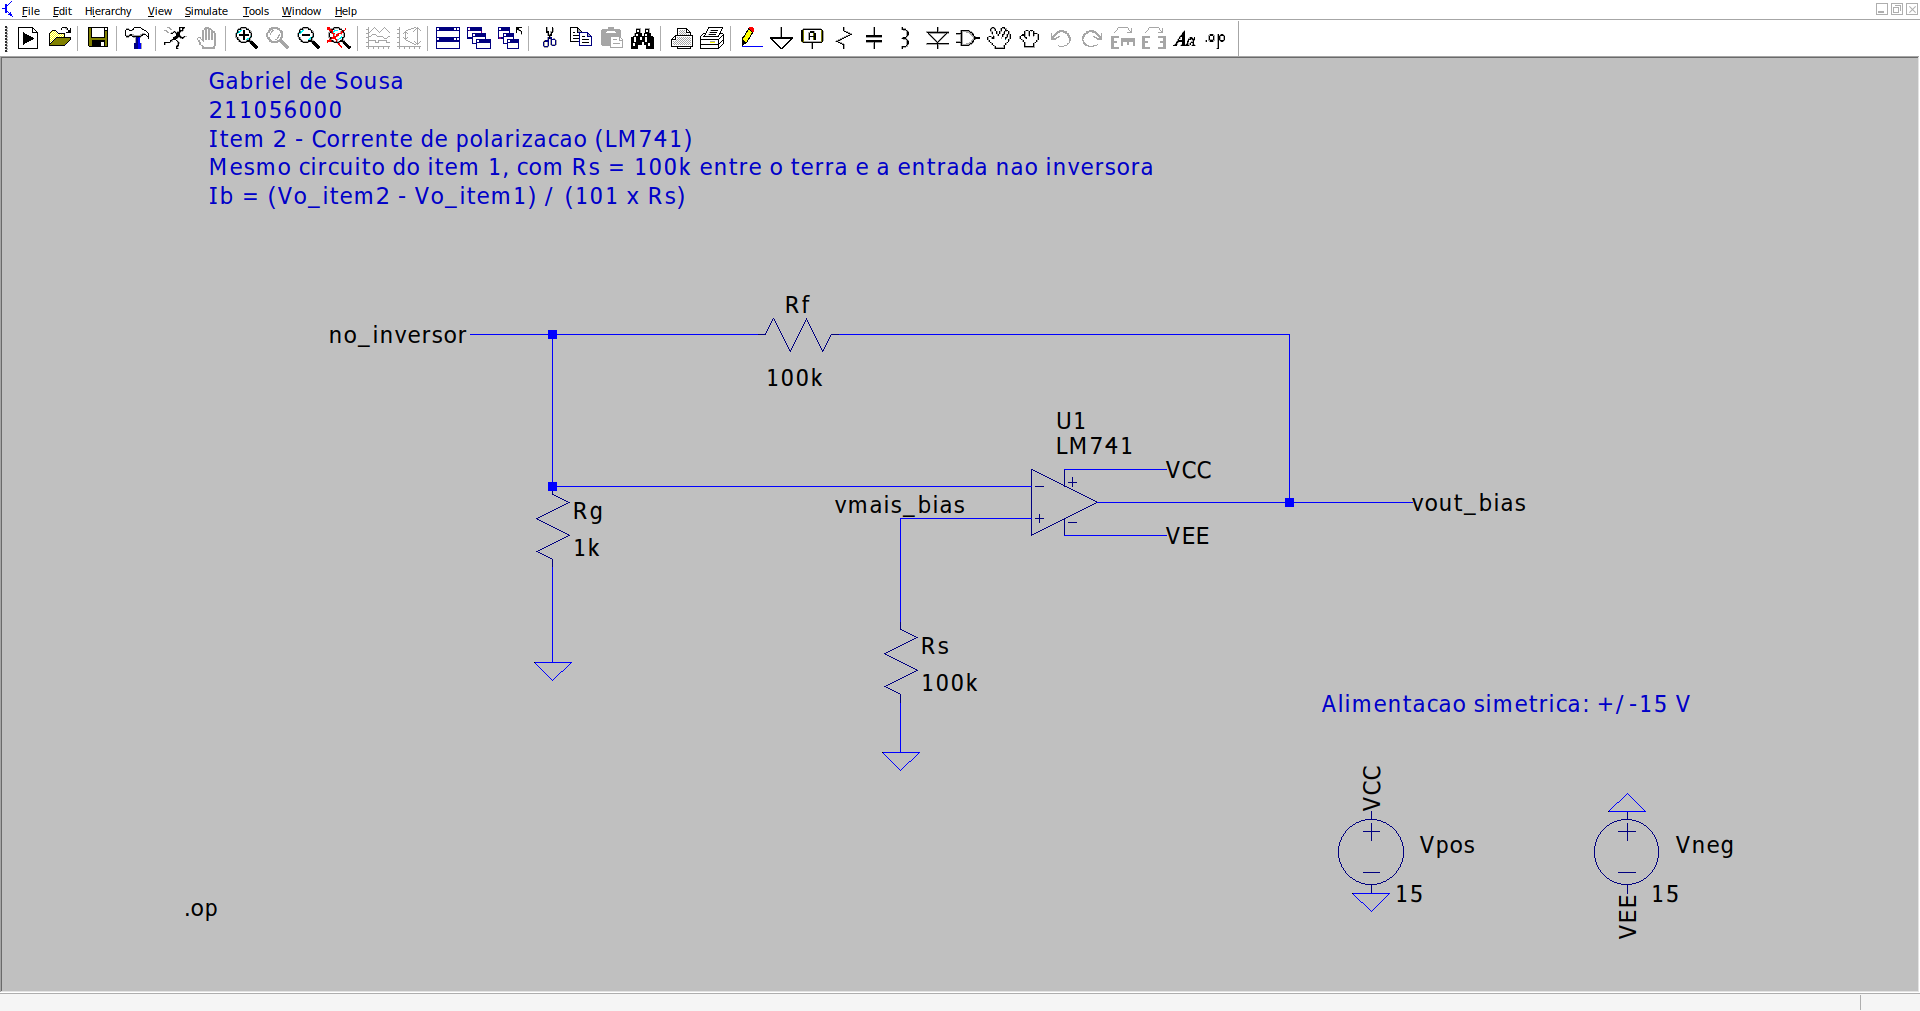
\includegraphics[width=\linewidth]{gabriel/item_2_circuito.png}
\caption{Gabriel, item\_2: circuito para obter \(I_b\) pela diferença de saída em relação ao item\_1.}
\label{fig:gabriel-item2}
\end{figure}

\paragraph{Item 3 — Resposta em frequência} Dois estágios independentes de ganhos nominais 34 e 119, com fonte comum \texttt{AC 1} e varredura \texttt{.ac dec 50 10 10meg}.

\begin{figure}[H]
\centering
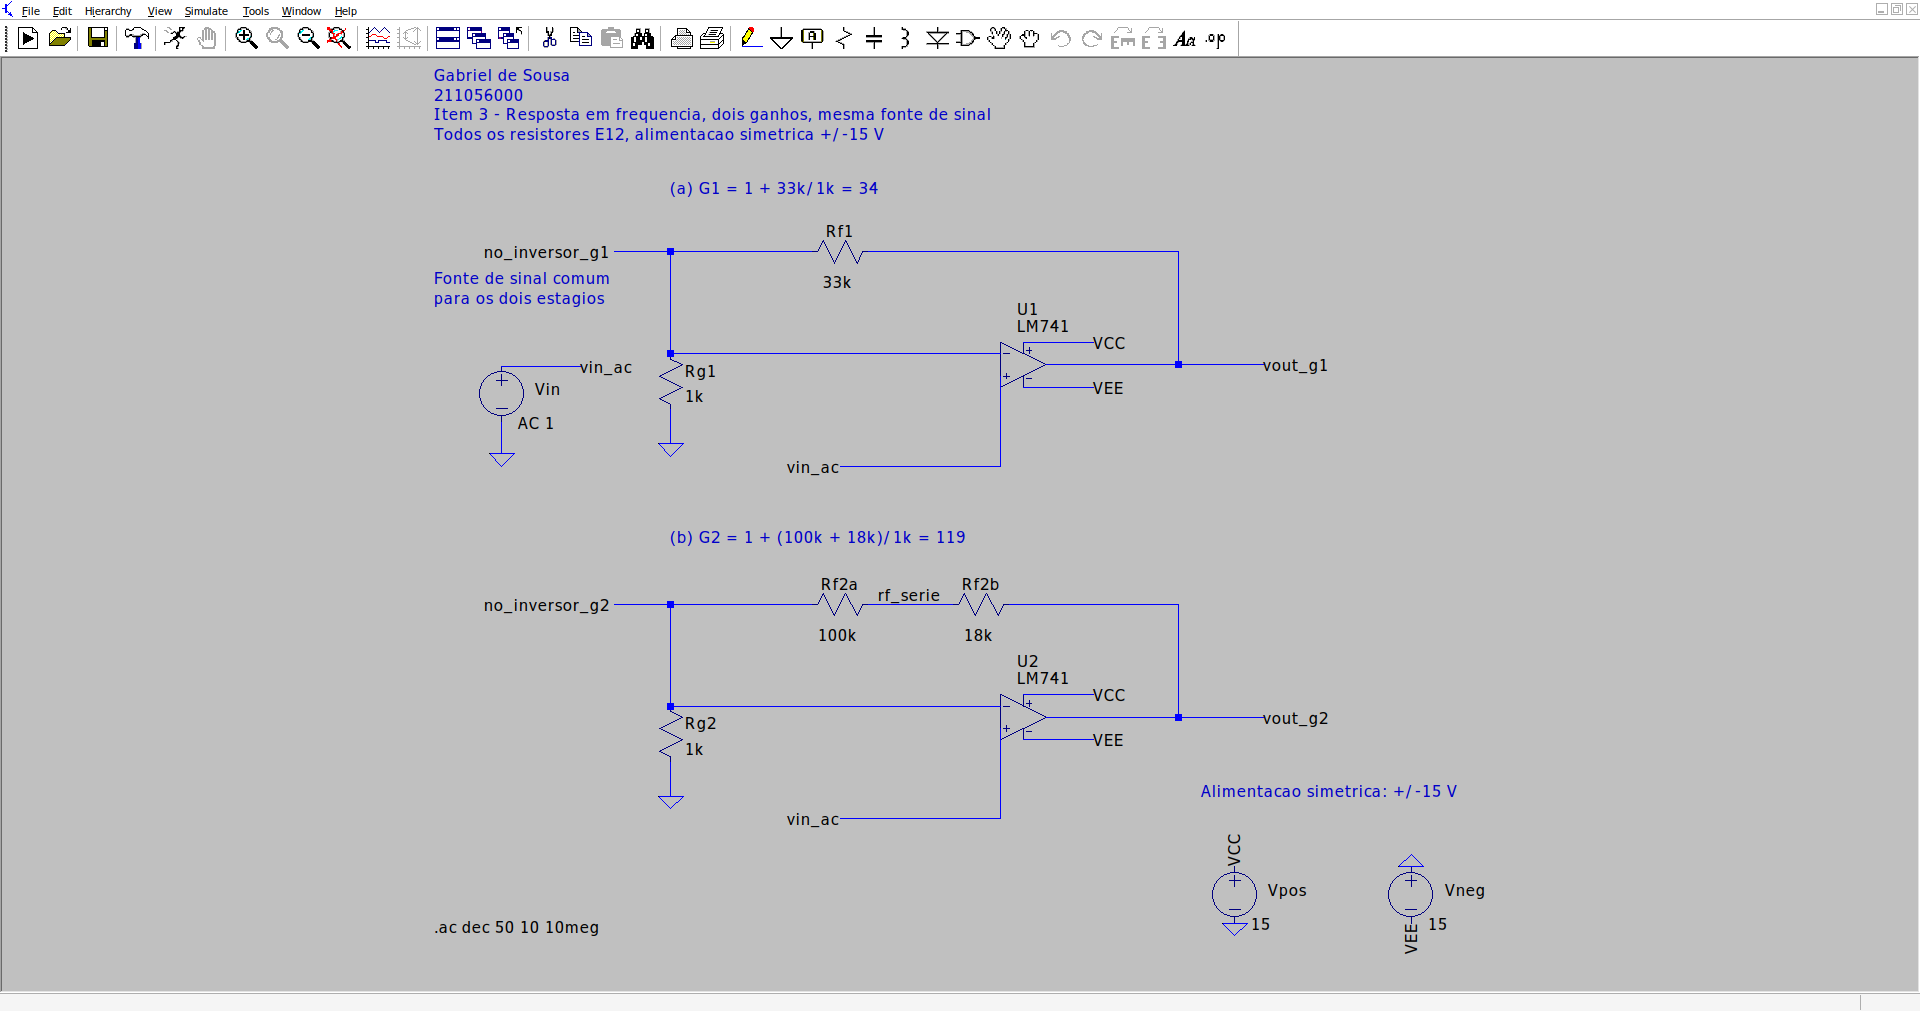
\includegraphics[width=\linewidth]{gabriel/item_3_circuito.png}
\caption{Gabriel, item\_3: os dois ganhos realizados com resistores E12.}
\label{fig:gabriel-item3}
\end{figure}

\paragraph{Item 4 — Slew rate do LM741} Seguidor com entrada de \(2\,\text{V}\) de pico, \texttt{.step} em \(5\) e \(100\,\text{kHz}\), dez períodos por frequência e passo máximo \(T/1000\). O arquivo usa integração Gear e \texttt{cshunt=0.01f}.

\begin{figure}[H]
\centering
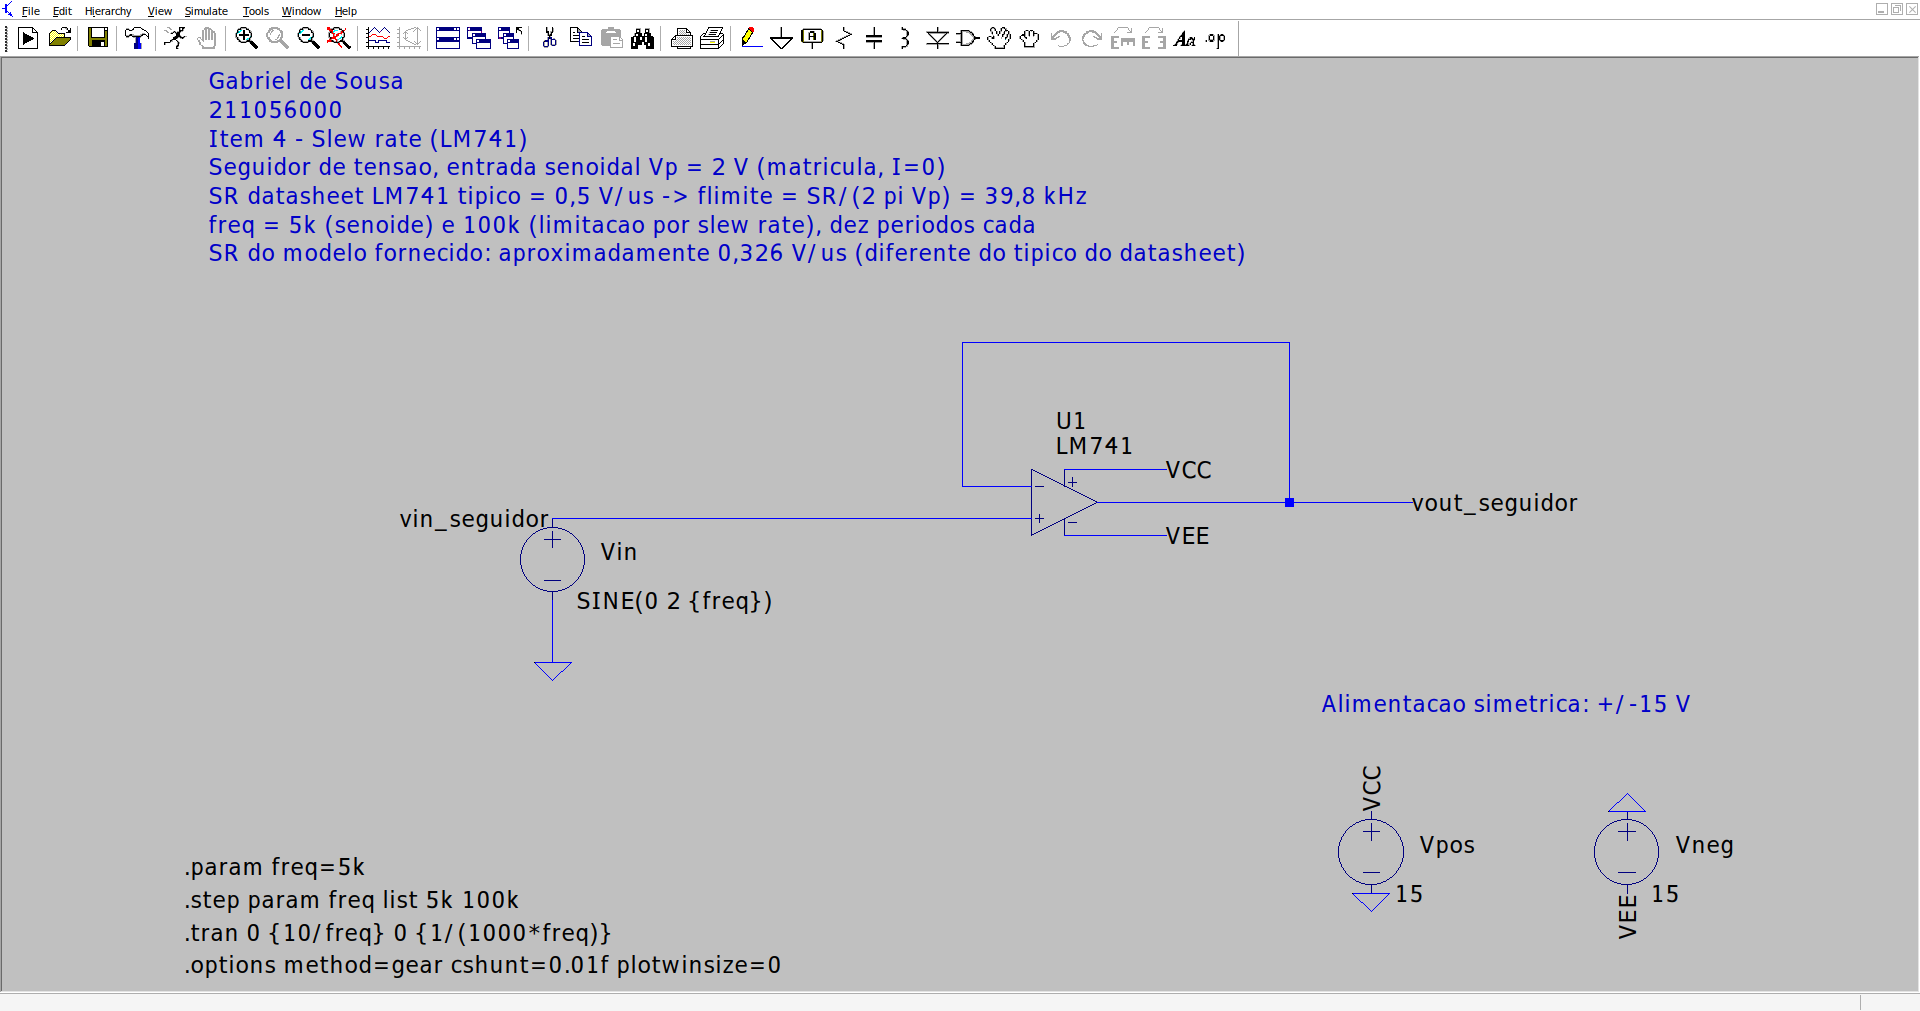
\includegraphics[width=\linewidth]{gabriel/item_4_circuito.png}
\caption{Gabriel, item\_4: seguidor com LM741 para observar a senoide e a limitação por slew rate.}
\label{fig:gabriel-item4}
\end{figure}

\paragraph{Item 5 — Corrente de polarização do TL064} Circuito do item\_2 com o TL064, mantendo os resistores e a análise \texttt{.op}. Para a subtração de saídas, também foi executada uma cópia auxiliar com o próprio TL064 e a entrada não inversora diretamente aterrada.

\begin{figure}[H]
\centering
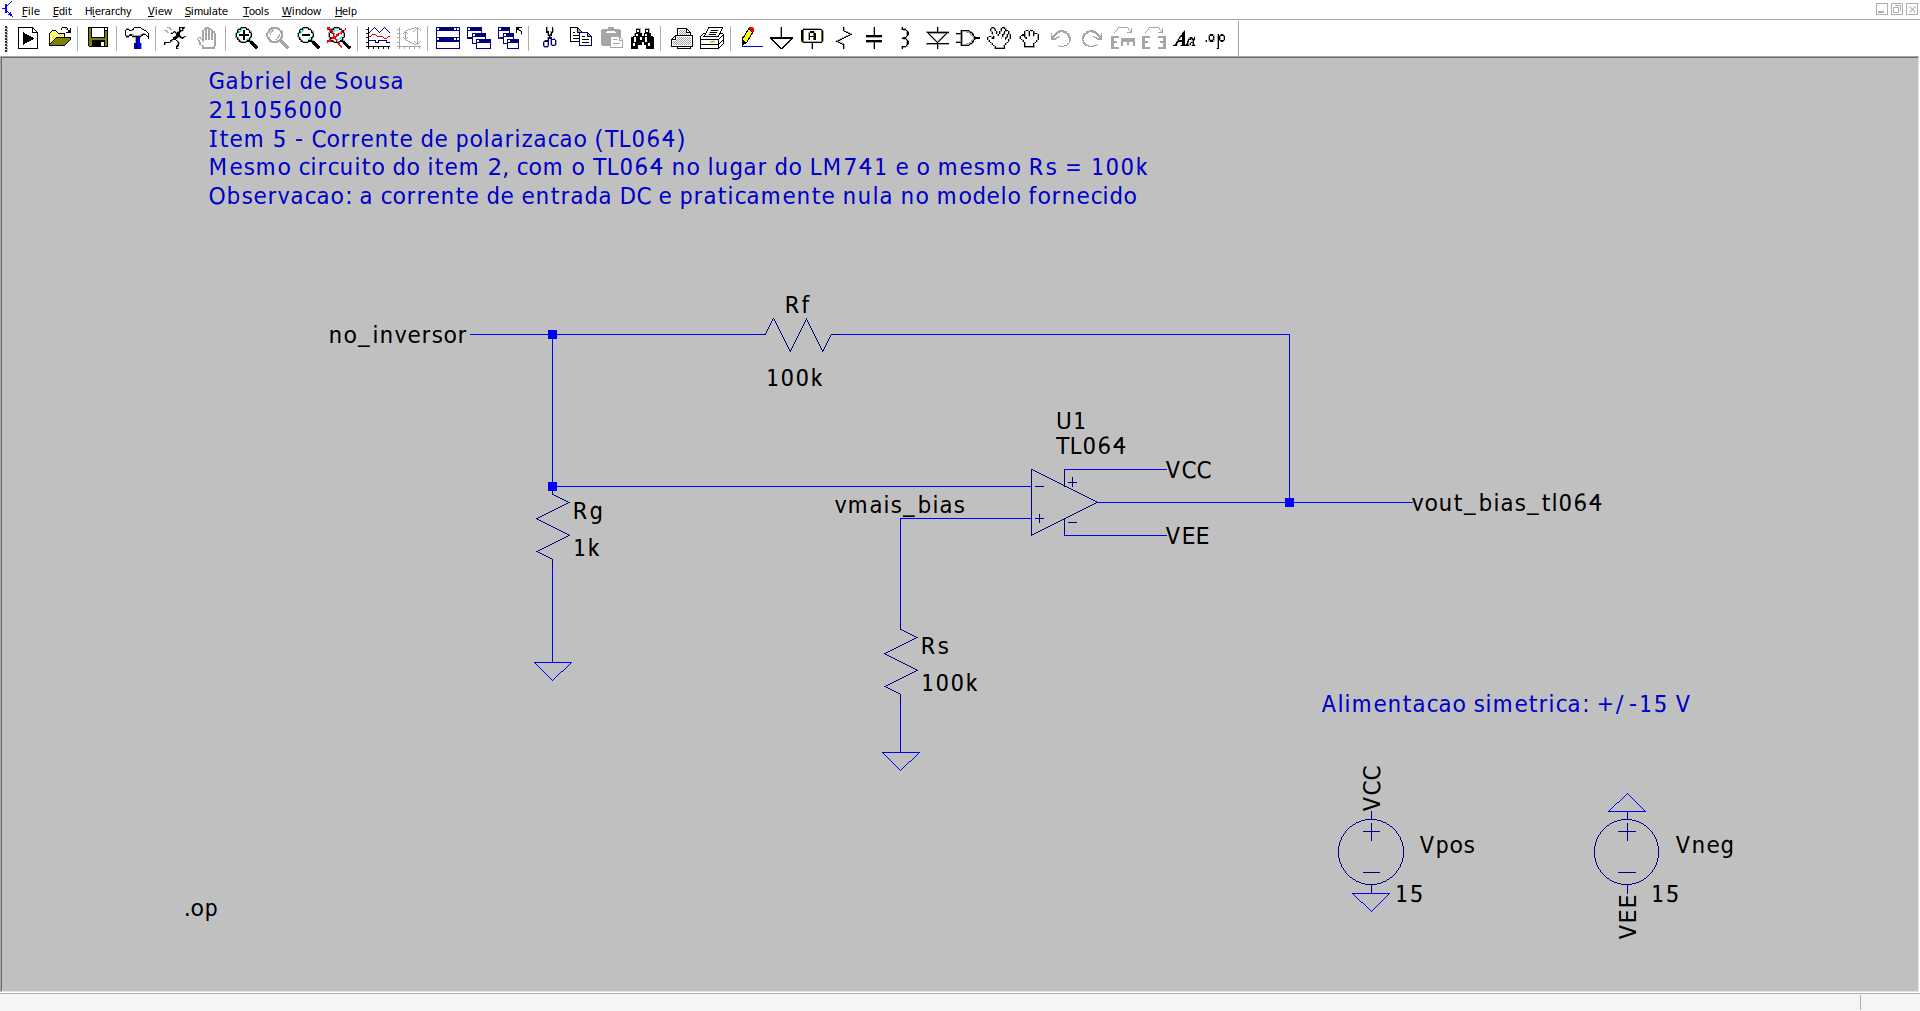
\includegraphics[width=\linewidth]{gabriel/item_5_circuito.png}
\caption{Gabriel, item\_5: medida de polarização com TL064; a referência de offset deve usar o mesmo modelo.}
\label{fig:gabriel-item5}
\end{figure}

\paragraph{Item 6 — Slew rate do TL064} Seguidor com entrada de \(2\,\text{V}\) de pico, frequências de \(50\) e \(500\,\text{kHz}\), dez períodos por frequência, integração Gear e passo máximo \(T/1000\).

\begin{figure}[H]
\centering
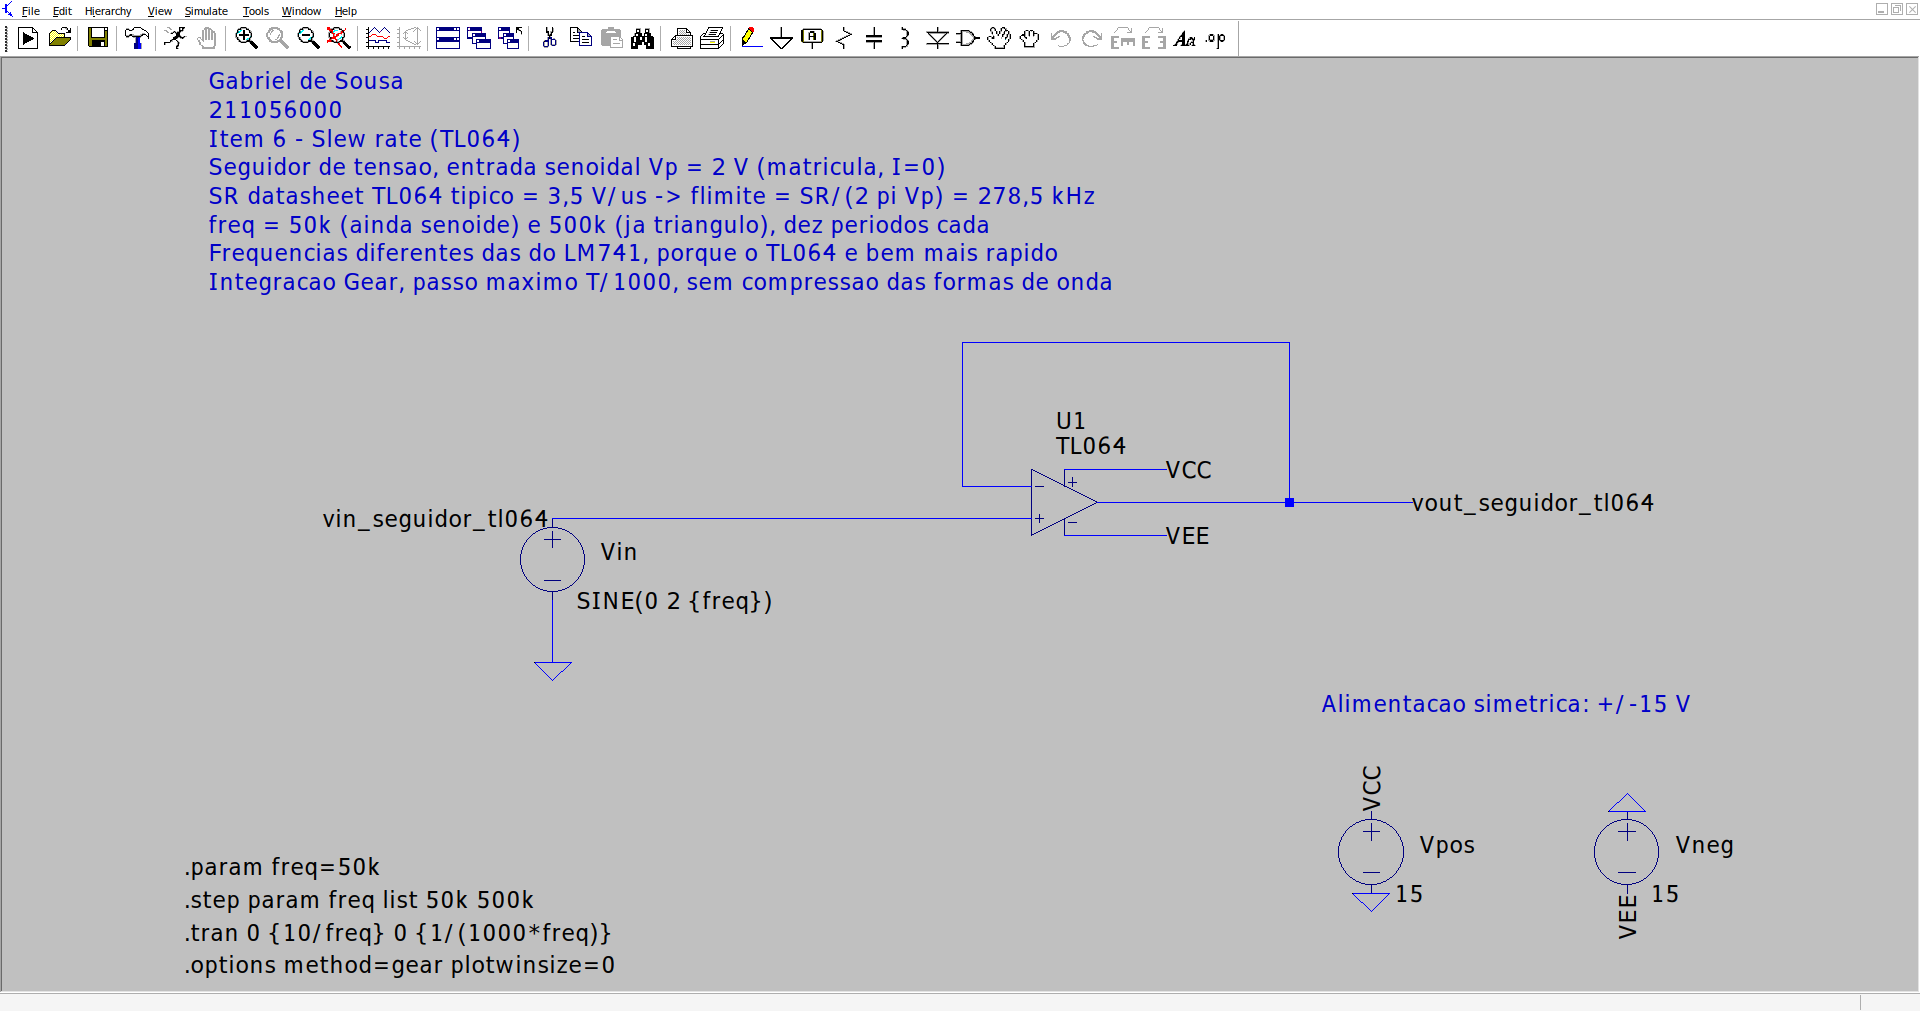
\includegraphics[width=\linewidth]{gabriel/item_6_circuito.png}
\caption{Gabriel, item\_6: seguidor com TL064, com frequências escolhidas para sua resposta mais rápida.}
\label{fig:gabriel-item6}
\end{figure}

\subsection{Montagem em bancada}
\label{sec:bancada}

A especificação de bancada é definida pelo número da equipe (Equipe~1), independente da
matrícula de qualquer integrante: ganho baixo \(G_1{=}11\) e amplitude de slew rate
\(V_p{=}2{,}0\,\text{V}\). O ganho alto é \(101\) para todas as equipes, com
\(R_f{=}100\,\text{k}\Omega\) e \(R_g{=}1\,\text{k}\Omega\) — o mesmo circuito serve às Seções~3.3,
3.4 e 3.5. Para o ganho baixo, entre os pares E12 exatos disponíveis na bancada
(\(1\text{k}/10\text{k}\), \(2{,}2\text{k}/22\text{k}\), \(10\text{k}/100\text{k}\)) foi escolhido
\(R_g{=}1\,\text{k}\Omega\), \(R_f{=}10\,\text{k}\Omega\), por reaproveitar o mesmo valor de
\(R_g\) já usado no ganho alto. A série de resistores do laboratório vai de \(820\,\Omega\) a
\(100\,\text{k}\Omega\), com no máximo um resistor por perna (sem combinações em série, diferente
da etapa de simulação).

\begin{center}\small
\setlength{\tabcolsep}{4pt}
\begin{tabular}{@{}llrr@{}}
\toprule
\textbf{Circuito} & \textbf{Componente} & \textbf{Nominal} & \textbf{Medido} \\
\midrule
Ganho alto (3.3/3.4/3.5) & \(R_f\) & \(100\,\text{k}\Omega\) & \(99{,}97\,\text{k}\Omega\) \\
Ganho alto (3.3/3.4/3.5) & \(R_g\) & \(1\,\text{k}\Omega\) & \(1{,}03\,\text{k}\Omega\) \\
Corrente de polarização (3.4) & \(R_s\) & \(100\,\text{k}\Omega\) & \(98{,}9\,\text{k}\Omega\) \\
Ganho baixo \(G_1{=}11\) (3.5) & \(R_f\) & \(10\,\text{k}\Omega\) & \(9{,}98\,\text{k}\Omega\) \\
Ganho baixo \(G_1{=}11\) (3.5) & \(R_g\) & \(1\,\text{k}\Omega\) & \(1{,}03\,\text{k}\Omega\)\footnotemark \\
\bottomrule
\end{tabular}
\end{center}
\footnotetext{Mesmo resistor físico do \(R_g\) do ganho alto, reaproveitado (Seção~\ref{sec:bancada}).}

Com esses valores, a Equação~\eqref{eq:naoinversor} dá o ganho realmente montado em cada estágio:
\(G_{\text{alto}}=1+99{,}97/1{,}03=98{,}058\) e \(G_{\text{baixo}}=1+9{,}98/1{,}03=10{,}689\).

O valor remedido de \(R_f\) do ganho baixo foi \(9{,}98\,\text{k}\Omega\).
O ganho calculado com os resistores medidos, \(10{,}689\), difere em \(5{,}6\%\) do
valor obtido pela razão entre as amplitudes no osciloscópio, \(11{,}324\).
Como os valores reais dos resistores já entram no cálculo, sua tolerância nominal não
explica novamente essa diferença; ela envolve a leitura das amplitudes, as condições
de montagem e as incertezas dos instrumentos. No ganho alto, a diferença entre
\(98{,}058\) calculado e \(98{,}336\) medido é de apenas \(0{,}28\%\).

A pinagem do LM741 (DIP de 8 pinos) e do TL064 (DIP de 14 pinos, usado só no amplificador~1,
pinos 1/2/3) segue o roteiro (Seção~3.2). A alimentação está \textbf{invertida} entre os dois
CIs: no LM741, \(V^-\) é o pino~4 e \(V^+\) é o pino~7; no TL064, \(V^+\) é o pino~4 e \(V^-\) é o
pino~11 — o erro mais fácil de cometer na troca de peça, e conferido a cada troca. O gerador foi
configurado para carga de alta impedância em toda a bancada, conforme o roteiro pede, sob pena de
entregar metade da tensão indicada no painel. O roteiro especifica capacitores de desacoplamento de \(100\,\text{nF}\) entre cada
alimentação e o terra. O registro da montagem documenta apenas o capacitor de
\(100\,\text{nF}\) entre a saída e o terra no ensaio de offset, usado para estabilizar a
leitura do multímetro. Esse capacitor não desempenha a função de desacoplamento das fontes.

A montagem seguiu a ordem do roteiro (Seção~3.7): alimentação e não inversor de ganho \(101\)
primeiro, com offset e corrente de polarização medidos só com o multímetro; depois o segundo
não inversor (ganho \(11\)), com o gerador e o osciloscópio para a resposta em frequência dos
dois estágios; em seguida a realimentação de um dos estágios foi desmontada para o ensaio de
slew rate; e por fim o LM741 foi trocado pelo TL064 para repetir a corrente de polarização e o
seguidor de tensão.

\begin{figure}[H]
\centering
\includegraphics[width=0.32\linewidth]{bancada/circuito_3.3.png}\hfill
\includegraphics[width=0.32\linewidth]{bancada/Vo_amp1_3.3.png}\hfill
\includegraphics[width=0.32\linewidth]{bancada/Vo_amp2_3.3.png}
\caption{Tensão de offset montada na bancada (LM741, ganho \(101\)) e as duas leituras do
multímetro: o primeiro LM741 (\(15{,}306\,\text{mV}\)) e o segundo, trocado no mesmo circuito
(\(16{,}339\,\text{mV}\)).}
\label{fig:bancada-33}
\end{figure}

\begin{figure}[H]
\centering
\includegraphics[width=0.32\linewidth]{bancada/Vo_LM741_Rs_3.4.png}\hfill
\includegraphics[width=0.32\linewidth]{bancada/Vo_TL064_fio_3.4.png}\hfill
\includegraphics[width=0.32\linewidth]{bancada/Vo_TL064_Rs_3.4.png}
\caption{Corrente de polarização: multímetro com o LM741 e \(R_s{=}100\,\text{k}\Omega\)
(\(-472{,}332\,\text{mV}\)), e as duas leituras do TL064 (fio, \(2{,}792\,\text{mV}\); com
\(R_s\), \(2{,}632\,\text{mV}\)). O registro desta seção é composto pelas leituras de multímetro.}
\label{fig:bancada-34}
\end{figure}

\begin{figure}[H]
\centering
\includegraphics[width=0.47\linewidth]{bancada/circuito_3.5_estagioA.png}\hfill
\includegraphics[width=0.47\linewidth]{bancada/circuito_3.5_estagioB.png}
\caption{Os dois estágios da resposta em frequência montados ao mesmo tempo: estágio A (ganho
\(101\), à esquerda) e estágio B (ganho \(11\), à direita), cada um com seu próprio LM741.}
\label{fig:bancada-35-circuito}
\end{figure}

\begin{figure}[H]
\centering
\includegraphics[width=0.47\linewidth]{bancada/osc_G11_ref_100Hz.png}\hfill
\includegraphics[width=0.47\linewidth]{bancada/osc_G101_ref_100Hz.png}
\caption{Referência em \(100\,\text{Hz}\) para os dois ganhos, com a saída (CH2, verde) ajustada
para \(2{,}00\,\text{V}_{pp}\) (\(1\,\text{V}\) de pico): ganho \(11\) (à esquerda,
\(181{,}03\,\text{mV}_{pp}\) de entrada) e ganho \(101\) (à direita,
\(19{,}83\,\text{mV}_{pp}\) de entrada).}
\label{fig:bancada-35-ref}
\end{figure}

\begin{figure}[H]
\centering
\includegraphics[width=0.47\linewidth]{bancada/osc_G11_corte_91kHz.png}\hfill
\includegraphics[width=0.47\linewidth]{bancada/osc_G11_triangulo_60kHz.png}
\caption{Ganho \(11\): registro em \(91{,}00\,\text{kHz}\), com saída de
\(1{,}48\,\text{V}_{pp}\) (à esquerda), e em \(60{,}00\,\text{kHz}\) (à direita).
A tabela de medições classifica os dois pontos como triangulares; a queda de amplitude
nesse regime não identifica isoladamente o corte linear.}
\label{fig:bancada-35-g11}
\end{figure}

\begin{figure}[H]
\centering
\includegraphics[width=0.55\linewidth]{bancada/osc_G101_corte_9p9kHz.png}
\caption{Ganho \(101\) em \(9{,}900\,\text{kHz}\): a saída caiu só para \(1{,}48\,\text{V}_{pp}\)
(razão de \(0{,}845\) com a referência, não os \(0{,}707\) do corte) — a entrada também caiu de
\(19{,}83\) para \(17{,}8\,\text{mV}_{pp}\) entre as duas capturas, então este ponto ainda não é
o corte real (ver Seção~\ref{sec:discussao}).}
\label{fig:bancada-35-g101}
\end{figure}

\begin{figure}[H]
\centering
\includegraphics[width=0.47\linewidth]{bancada/circuito_3.6_LM741.png}\hfill
\includegraphics[width=0.47\linewidth]{bancada/circuito_3.6_TL064.png}
\caption{Seguidor de tensão para o slew rate: LM741 (à esquerda, sem \(R_f\) nem \(R_g\)) e
TL064 (à direita, amplificador~1, pino~1 realimentado direto ao pino~2).}
\label{fig:bancada-36-circuito}
\end{figure}

\begin{figure}[H]
\centering
\includegraphics[width=0.47\linewidth]{bancada/osc_LM741_triangulo.png}\hfill
\includegraphics[width=0.47\linewidth]{bancada/osc_LM741_cursores.png}
\caption{Slew rate do LM741: triângulo em \(39{,}7\,\text{kHz}\) (à esquerda) e a mesma rampa com
os cursores do osciloscópio (à direita), \(\Delta V{=}2{,}47\,\text{V}\),
\(\Delta t{=}7{,}860\,\mu\text{s}\), \(SR{=}0{,}314\,\text{V}/\mu\text{s}\).}
\label{fig:bancada-36-lm741}
\end{figure}

\begin{figure}[H]
\centering
\includegraphics[width=0.47\linewidth]{bancada/osc_TL064_triangulo.png}\hfill
\includegraphics[width=0.47\linewidth]{bancada/osc_TL064_cursores.png}
\caption{Slew rate do TL064: triângulo em \(447{,}0\,\text{kHz}\) (à esquerda) e a rampa com
cursores (à direita), \(\Delta V{=}2{,}74\,\text{V}\), \(\Delta t{=}0{,}796\,\mu\text{s}\),
\(SR{=}3{,}442\,\text{V}/\mu\text{s}\).}
\label{fig:bancada-36-tl064}
\end{figure}

\subsection{Simulação da montagem}
\label{sec:sim-montagem}

Os circuitos de offset e polarização foram simulados em ponto de operação com
\(R_f=99{,}97\,\text{k}\Omega\), \(R_g=1{,}03\,\text{k}\Omega\) e,
quando presente, \(R_s=98{,}9\,\text{k}\Omega\). O capacitor de saída usado no ensaio
de offset não altera o ponto de operação ideal, pois se comporta como circuito aberto
em corrente contínua. A resposta em frequência foi simulada com dois LM741:
\(R_f=9{,}98\,\text{k}\Omega\) no estágio baixo e \(99{,}97\,\text{k}\Omega\)
no alto, ambos com \(R_g=1{,}03\,\text{k}\Omega\).

Foram mantidos os macromodelos da disciplina, a alimentação de \(\pm15\,\text{V}\)
e a temperatura padrão do simulador, \(27\,^{\circ}\text{C}\).
A análise AC representa pequeno sinal; não reproduz a distorção por slew rate.
Os ensaios transientes usam \(V_p=2\,\text{V}\), referência de \(1\,\text{kHz}\)
e as frequências registradas nos ensaios triangulares: \(39{,}7\,\text{kHz}\) no LM741
e \(447\,\text{kHz}\) no TL064. Foram simulados dez períodos por frequência, com
passo máximo \(T/1000\), integração Gear e sem compressão. O ensaio do LM741 mantém
\texttt{cshunt=0.01f}, como no projeto individual. Fontes e interligações são ideais;
parasitismos do protoboard e incertezas instrumentais não estão incluídos.

\begin{center}\small
\setlength{\tabcolsep}{4pt}
\begin{tabular}{@{}lrr@{}}
\toprule
\textbf{Grandeza} & \textbf{Simulação da montagem} & \textbf{Bancada} \\
\midrule
LM741, saída sem \(R_s\) & \(108{,}189\,\text{mV}\) & \(15{,}306\,\text{mV}\) (nº1) \\
LM741, saída com \(R_s\) & \(-452{,}581\,\text{mV}\) & \(-472{,}332\,\text{mV}\) \\
LM741, \(\Delta V_o\) & \(-560{,}770\,\text{mV}\) & \(-487{,}638\,\text{mV}\) \\
LM741, \(\lvert I_b\rvert\) & \(57{,}824\,\text{nA}\) & \(50{,}3\,\text{nA}\) \\
TL064, saída sem \(R_s\) & \(2{,}62514\,\text{mV}\) & \(2{,}792\,\text{mV}\) \\
TL064, saída com \(R_s\) & \(2{,}62514\,\text{mV}\) & \(2{,}632\,\text{mV}\) \\
Ganho baixo & \(10{,}689\) & \(11{,}324\) \\
Ganho alto & \(98{,}013\) & \(98{,}336\) \\
Corte linear, ganho baixo & \(96{,}00\,\text{kHz}\) & distorção na varredura \\
Corte, ganho alto & \(10{,}20\,\text{kHz}\) & \(15{,}50\,\text{kHz}\) (ajuste) \\
\(Gf_c\), ganho baixo & \(1{,}0262\,\text{MHz}\) & não isolado \\
\(Gf_c\), ganho alto & \(0{,}9997\,\text{MHz}\) & \(1{,}524\,\text{MHz}\) (ajuste) \\
\(SR\), LM741 & \(0{,}3252\,\text{V}/\mu\text{s}\) & \(0{,}314\,\text{V}/\mu\text{s}\) \\
\(SR\), TL064 & \(3{,}4848\,\text{V}/\mu\text{s}\) & \(3{,}442\,\text{V}/\mu\text{s}\) \\
\bottomrule
\end{tabular}
\end{center}

Os ganhos simulados são obtidos no início da varredura AC; os experimentais são as
razões de amplitudes em \(100\,\text{Hz}\). A estimativa de corte por ajuste usa os
pontos experimentais completos descritos na Seção~\ref{sec:freq-bancada}.
Os slew rates simulados são as médias dos módulos das rampas de subida e descida,
obtidas por ajuste linear para \(\lvert V_{out}\rvert<0{,}2\,\text{V}\) no último período.

Para calcular as grandezas de entrada a partir da bancada, foi usado
\(G=1+99{,}97/1{,}03=98{,}058\). Resultam
\(V_{os,1}=15{,}306/98{,}058=0{,}1561\,\text{mV}\) e
\(V_{os,2}=16{,}339/98{,}058=0{,}1666\,\text{mV}\).
Para a polarização, \(I_b=\Delta V_o/(98{,}058\times98{,}9\,\text{k}\Omega)\),
resultando em módulos de \(50{,}3\,\text{nA}\) e \(16{,}5\,\text{pA}\).
A simulação fornece \(V_o/G=1{,}1033\,\text{mV}\) no LM741 e corrente aproximadamente
nula no TL064, limitada pela representação DC de suas entradas no macromodelo.

\begin{figure}[H]
\centering
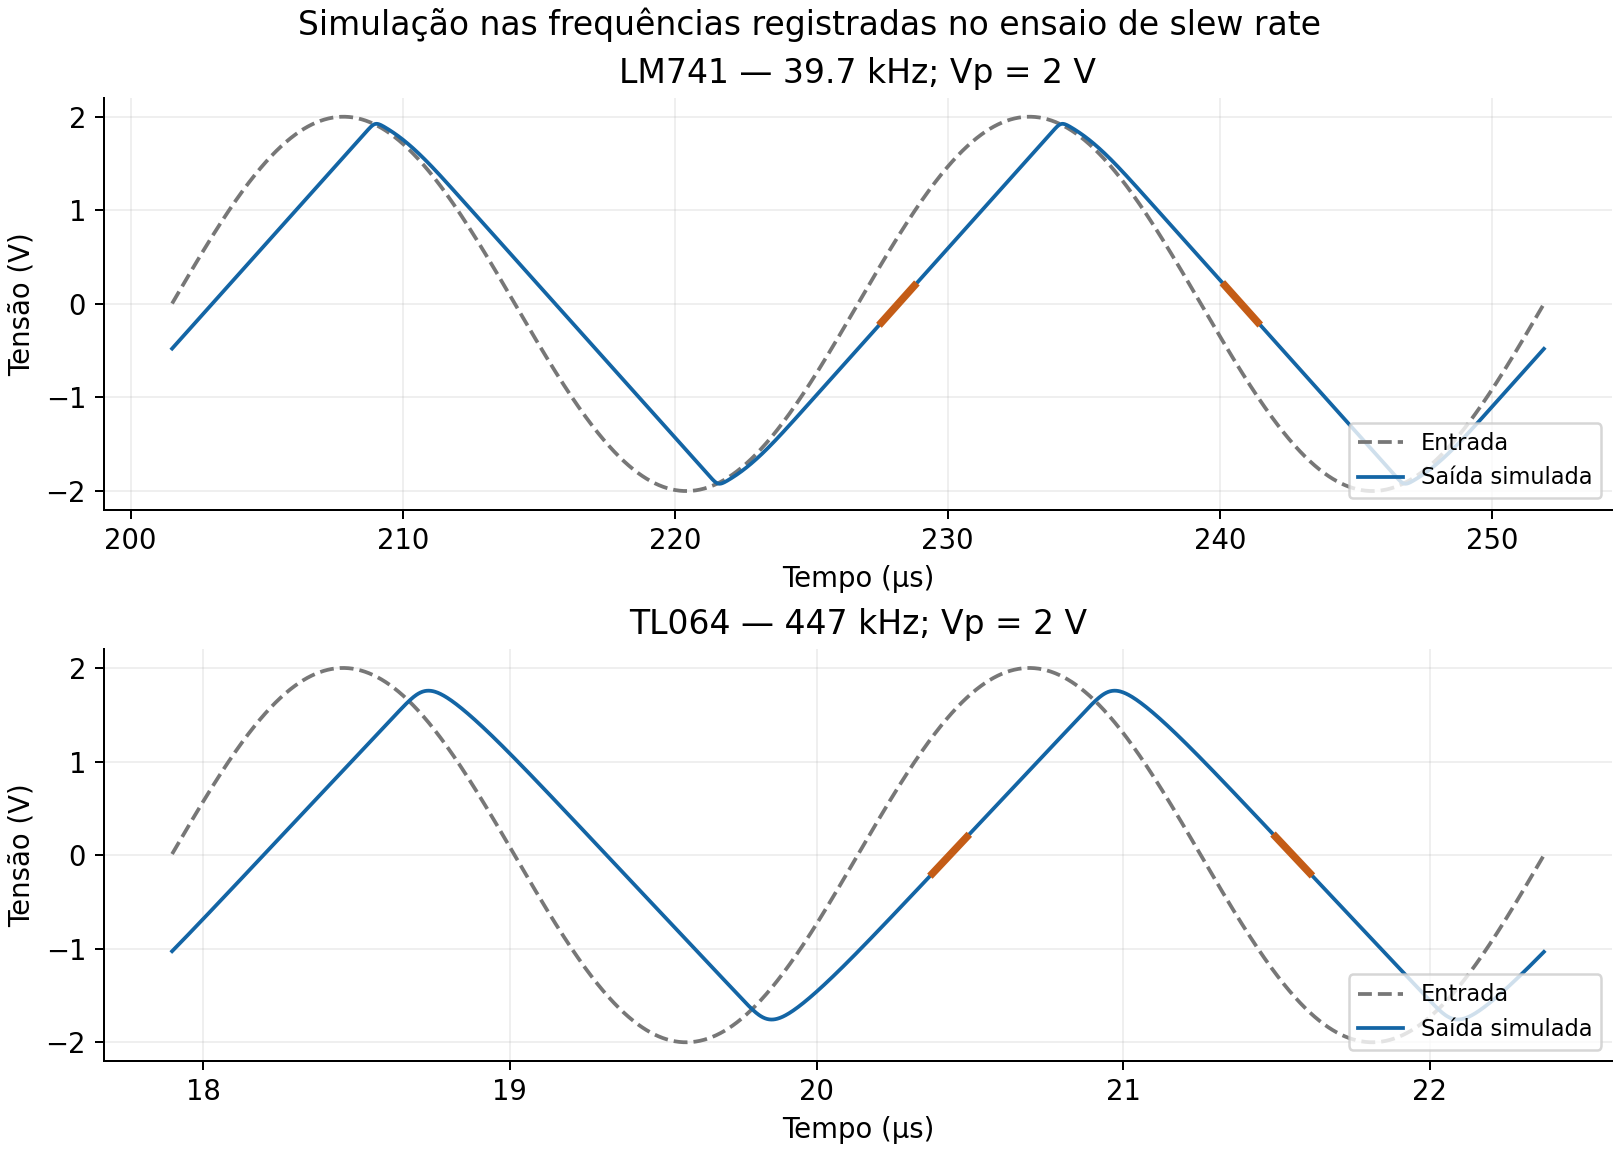
\includegraphics[width=\linewidth]{gabriel/montagem_slew.png}
\caption{Simulação da montagem nas frequências do ensaio de slew rate, com entrada de
\(2\,\text{V}\) de pico. São apresentados os dois últimos períodos; os trechos em
laranja foram usados para medir as rampas.}
\label{fig:montagem-slew}
\end{figure}

\section{Resultados}
\label{sec:resultados}

\subsection{Projeto de cada integrante}
\label{sec:resultados-projeto}

\textbf{Ana Luísa Reis Nascente.} Valores já deduzidos na Seção~\ref{sec:espec} (Teórico =
especificação; Simulado = resultado do LTspice com os componentes escolhidos):

\begin{center}\small
\setlength{\tabcolsep}{4pt}
\begin{tabular}{@{}llrrr@{}}
\toprule
\textbf{Item} & \textbf{Grandeza} & \textbf{Teórico} & \textbf{Simulado} & \textbf{Desvio} \\
\midrule
1 & \(V_{os}\) (LM741) & — & \(1{,}1003\,\text{mV}\) & — \\
2 & \(I_b\) (LM741) & — & \(57{,}82\,\text{nA}\) & — \\
3 & \(G_1\) realizado & \(23{,}000\) & \(23{,}000\) & \(0{,}00\%\) \\
3 & \(G_2\) realizado & \(107{,}00\) & \(106{,}833\) & \(-0{,}16\%\) \\
3 & Corte, estágio \(G_1\) & — & \(43{,}82\,\text{kHz}\) & — \\
3 & Corte, estágio \(G_2\) & — & \(9{,}33\,\text{kHz}\) & — \\
3 & \(G\times\)corte, estágio \(G_1\) & \({\approx}1\,\text{MHz}\) (GBW) & \(1{,}008\,\text{MHz}\) & \(+0{,}8\%\) \\
3 & \(G\times\)corte, estágio \(G_2\) & \({\approx}1\,\text{MHz}\) (GBW) & \(0{,}997\,\text{MHz}\) & \(-0{,}3\%\) \\
4 & SR (LM741) & — & \(0{,}320\,\text{V}/\mu\text{s}\) & — \\
5 & \(I_b\) (TL064) & — & \({\approx}0\) & — \\
6 & SR (TL064) & — & \(3{,}43\,\text{V}/\mu\text{s}\) & — \\
\bottomrule
\end{tabular}
\end{center}

Os três gráficos abaixo mostram o comportamento por trás desses números — o que o roteiro pede
para "observar", não só para tabular.

\begin{figure}[H]
\centering
\includegraphics[width=0.85\linewidth]{ana/item_3_grafico.png}
\caption{Resposta em frequência simulada do item\_3: ganho em dB (eixo vertical) contra
frequência em escala log (eixo horizontal), uma curva para \(G_1{=}23\) e outra para
\(G_2{\approx}106{,}8\).}
\label{fig:item3-grafico}
\end{figure}

A Figura~\ref{fig:item3-grafico} é o retrato direto da Equação~\eqref{eq:corte}: as duas curvas
partem de um patamar plano em baixa frequência — \(27{,}234\,\text{dB}\) (\({\approx}23\,\text{V/V}\))
para \(G_1\) e \(40{,}570\,\text{dB}\) (\({\approx}106{,}8\,\text{V/V}\)) para \(G_2\), a
diferença entre os dois patamares sendo exatamente \(20\log_{10}(106{,}8/23)=13{,}3\,\text{dB}\)
— e cada uma cai à taxa de \(-20\,\text{dB}/\text{década}\) a partir do seu próprio corte
(\(43{,}82\,\text{kHz}\) para \(G_1\), bem mais adiante no eixo que os \(9{,}33\,\text{kHz}\) de
\(G_2\)). O detalhe mais informativo do gráfico é o que acontece em alta frequência: as duas
curvas, apesar de partirem de patamares tão diferentes, convergem para a mesma reta de
\(-20\,\text{dB}/\text{década}\) — a envoltória de malha aberta do próprio LM741. É a prova
visual de que o produto \(G\times f_c\) é uma constante do dispositivo (o GBW), não um artefato de
cada malha de realimentação: usando a Equação~\eqref{eq:corte} com o GBW típico de
\({\approx}1\,\text{MHz}\), o corte previsto seria \(1\,\text{MHz}/23{\approx}43{,}5\,\text{kHz}\)
e \(1\,\text{MHz}/106{,}8{\approx}9{,}36\,\text{kHz}\) — a \(0{,}7\%\) e \(0{,}3\%\) dos cortes
que o LTspice realmente simulou. Na bancada, a comparação exige distinguir pequeno sinal de distorção por slew rate,
como discutido na Seção~\ref{sec:freq-bancada}.

\begin{figure}[H]
\centering
\includegraphics[width=0.85\linewidth]{ana/item_4_grafico.png}
\caption{Slew rate simulado do LM741 (item\_4): \(V_{out}\) contra o tempo, sobrepondo as duas
frequências do \texttt{.step} (\(5\,\text{kHz}\) e \(50\,\text{kHz}\)) para a mesma amplitude de
entrada \(V_p{=}6\,\text{V}\).}
\label{fig:item4-grafico}
\end{figure}

Na Figura~\ref{fig:item4-grafico}, a curva de maior amplitude é a senoide de \(5\,\text{kHz}\):
ela ocupa toda a excursão de \(\pm6\,\text{V}\) e mantém o formato arredondado de uma senoide do
início ao fim dos dez períodos simulados, porque a taxa de variação que ela pede
(\(2\pi\times5\,\text{kHz}\times6\,\text{V}{\approx}0{,}19\,\text{V}/\mu\text{s}\), pela
Equação~\eqref{eq:slew-taxa}) fica bem abaixo do \(SR{\approx}0{,}32\,\text{V}/\mu\text{s}\)
simulado do LM741. A segunda curva, muito mais rápida e de amplitude visivelmente menor, é a de
\(50\,\text{kHz}\): nessa frequência a taxa pedida
(\(2\pi\times50\,\text{kHz}\times6\,\text{V}{\approx}1{,}88\,\text{V}/\mu\text{s}\)) é quase seis
vezes o \(SR\) disponível, então o AmpOp já não consegue completar a subida ou a descida dentro
de meio período: a tensão sobe e desce à taxa constante do slew rate em vez de acompanhar a
senoide, achatando o pico (\({\approx}{+}2{,}7\,\text{V}/{-}1{,}7\,\text{V}\), bem aquém dos
\(\pm6\,\text{V}\) pedidos) e transformando a forma de onda num triângulo com os lados retos
característicos de uma rampa a taxa constante. É exatamente esse mecanismo — não uma atenuação de
amplitude linear, mas uma saturação na \emph{taxa} de subida — que a bancada reproduziu na
Seção~3.6: o \(SR\) medido lá (\(0{,}314\,\text{V}/\mu\text{s}\)) é quase idêntico ao
\(0{,}320\,\text{V}/\mu\text{s}\) simulado aqui, e o triângulo apareceu na bancada já em
\(39{,}7\,\text{kHz}\) (com \(V_p{=}2\,\text{V}\) de bancada, um limiar mais alto que aqui porque
o limiar da Equação~\eqref{eq:slew-fmax} é inversamente proporcional à amplitude).

\begin{figure}[H]
\centering
\includegraphics[width=0.85\linewidth]{ana/item_6_grafico.png}
\caption{Slew rate simulado do TL064 (item\_6): mesmo formato do item\_4, agora com \texttt{.step}
entre \(5\,\text{kHz}\) e \(500\,\text{kHz}\).}
\label{fig:item6-grafico}
\end{figure}

A Figura~\ref{fig:item6-grafico} repete a mesma leitura com o TL064, e a diferença de escala já
salta aos olhos: foi preciso subir a segunda frequência para \(500\,\text{kHz}\) —
\(10\times\) mais alta que no LM741 — só para começar a ver o mesmo tipo de achatamento e
distorção da senoide em triângulo, porque o \(SR{\approx}3{,}43\,\text{V}/\mu\text{s}\) do TL064
tolera uma taxa de variação bem maior antes de saturar. Ainda assim, em \(500\,\text{kHz}\) a
curva rápida já perde a forma arredondada e a amplitude cai bem abaixo dos \(\pm6\,\text{V}\) da
senoide de \(5\,\text{kHz}\), mostrando que o mesmo mecanismo físico da Seção~\ref{sec:teoria}
(o capacitor de compensação interno carregando à corrente máxima disponível) está em ação, só que
numa faixa de frequência mais alta. O \(SR\) medido na bancada
(\(3{,}442\,\text{V}/\mu\text{s}\)) bate com o \(3{,}43\,\text{V}/\mu\text{s}\) simulado aqui a
menos de \(0{,}5\%\) de diferença, e o triângulo na bancada apareceu em \(447\,\text{kHz}\) — da
mesma ordem de grandeza dos \(500\,\text{kHz}\) usados nesta simulação, ainda que com uma
amplitude de teste diferente (\(V_p{=}2\,\text{V}\) na bancada contra \(6\,\text{V}\) aqui).

\textbf{Gabriel de Sousa.}
\label{sec:gabriel-resultados}
Os resultados abaixo correspondem aos arquivos apresentados na
Seção~\ref{sec:gabriel-simulacoes}. Os ganhos simulados são os valores de
\(\lvert V_{out}/V_{in}\rvert\) em \(10\,\text{Hz}\); os cortes foram interpolados
em frequência logarítmica na queda de \(3{,}0103\,\text{dB}\) em relação a esses valores.

\begin{center}\small
\setlength{\tabcolsep}{4pt}
\begin{tabular}{@{}llrr@{}}
\toprule
\textbf{Item} & \textbf{Grandeza} & \textbf{Projeto / referência} & \textbf{Simulado} \\
\midrule
1 & \(V_o\), LM741 sem \(R_s\) & — & \(111{,}131\,\text{mV}\) \\
1 & \(V_{os}=V_o/101\) & — & \(1{,}10031\,\text{mV}\) \\
2 & \(V_o'\), LM741 com \(R_s\) & — & \(-472{,}874\,\text{mV}\) \\
2 & \(\lvert I_b\rvert\), LM741 & — & \(57{,}822\,\text{nA}\) \\
3 & Ganho \(G_1\) & \(34\) & \(33{,}995\) \\
3 & Ganho \(G_2\) & \(119\) & \(118{,}933\) \\
3 & Corte de \(G_1\) & \(29{,}412\,\text{kHz}^{*}\) & \(29{,}580\,\text{kHz}\) \\
3 & Corte de \(G_2\) & \(8{,}403\,\text{kHz}^{*}\) & \(8{,}402\,\text{kHz}\) \\
3 & \(G_1f_{c1}\) & \(1\,\text{MHz}^{*}\) & \(1{,}0056\,\text{MHz}\) \\
3 & \(G_2f_{c2}\) & \(1\,\text{MHz}^{*}\) & \(0{,}9993\,\text{MHz}\) \\
4 & \(SR\), LM741 (módulo) & \(0{,}5\,\text{V}/\mu\text{s}^{\dagger}\) & \(0{,}3252\,\text{V}/\mu\text{s}\) \\
5 & \(V_o\), TL064 sem/com \(R_s\) & — & \(2{,}70260\,\text{mV}\) \\
5 & \(I_b\), TL064 & — & \({\approx}0\) (modelo) \\
6 & \(SR\), TL064 (módulo) & \(3{,}5\,\text{V}/\mu\text{s}^{\dagger}\) & \(3{,}493\,\text{V}/\mu\text{s}\) \\
\bottomrule
\end{tabular}
\end{center}
{\small \(^{*}\)Estimativa de um polo com GBW de referência de \(1\,\text{MHz}\).
\(^{\dagger}\)Valores típicos de datasheet usados no roteiro e nas anotações dos circuitos;
não são os valores impostos pelo macromodelo.}

No LM741, \(\Delta V_o=-584{,}005\,\text{mV}\), logo a Equação~\eqref{eq:bias}
fornece \(-57{,}822\,\text{nA}\): o sinal negativo nessa convenção indica corrente
entrando no pino não inversor. O offset coincide, no arredondamento, com o de Ana,
pois os dois ensaios usam o mesmo circuito e o mesmo modelo.

No TL064, as saídas com e sem \(R_s\) foram iguais na precisão dos dados gravados.
A corrente obtida pela subtração é, portanto, aproximadamente nula, como já indicado
no arquivo. Isso é uma limitação do macromodelo para a corrente DC de entrada, não
uma previsão de corrente exatamente nula na peça real. Não se extrai uma razão
finita confiável entre as correntes dos dois modelos dessa subtração.

\begin{figure}[H]
\centering
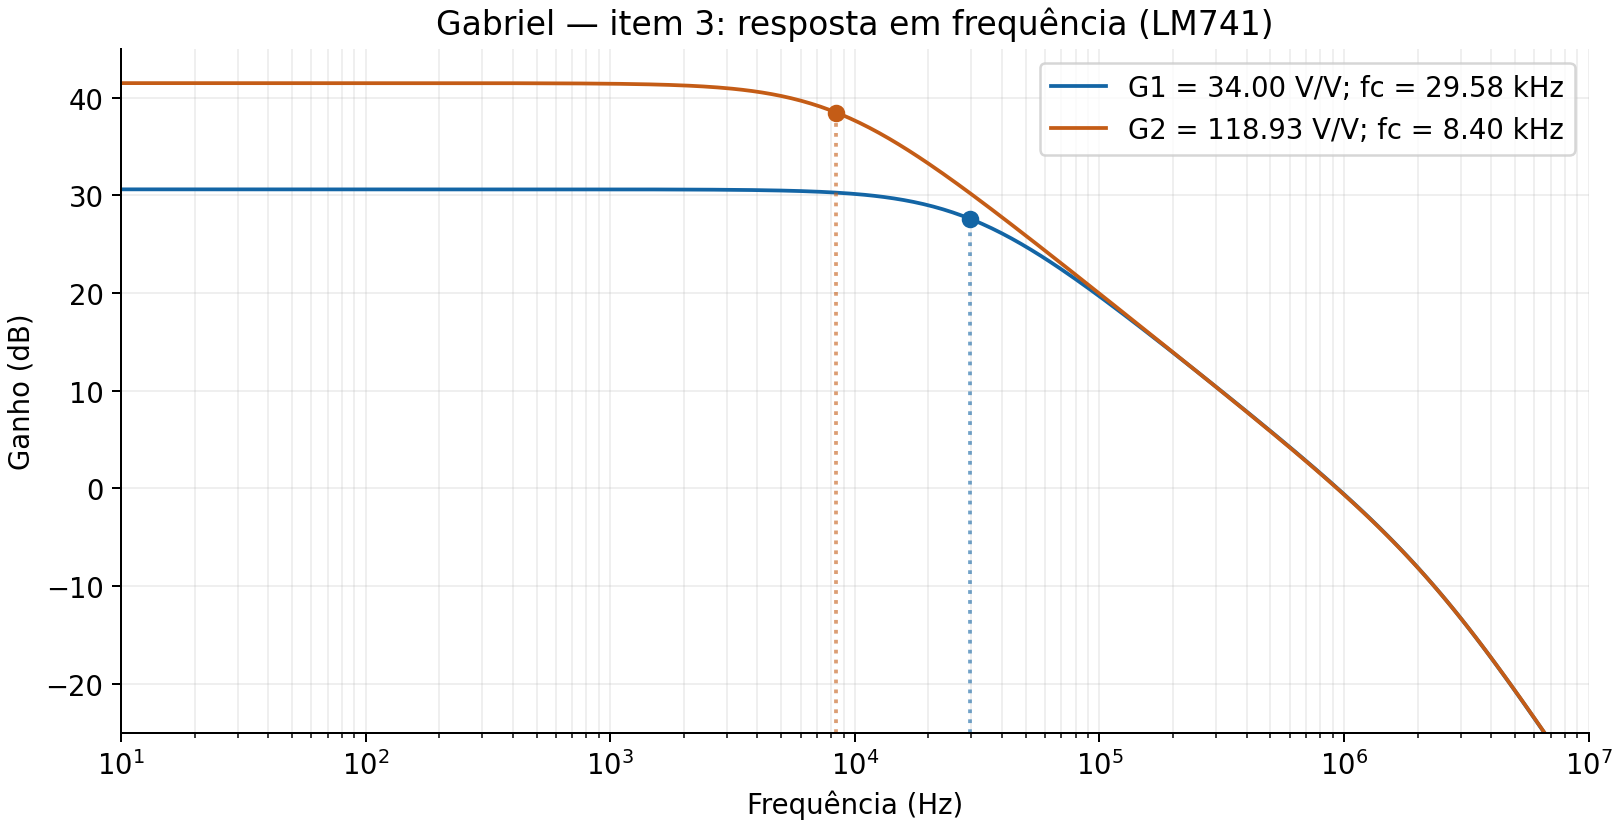
\includegraphics[width=\linewidth]{gabriel/item_3_grafico.png}
\caption{Gabriel, item\_3: resposta em frequência extraída da análise AC do LTspice.
Os pontos indicam os cortes relativos ao patamar de cada estágio.}
\label{fig:gabriel-item3-grafico}
\end{figure}

Os dois produtos ganho-corte diferem em cerca de \(0{,}63\%\), ambos próximos de
\(1\,\text{MHz}\). Comparados ao projeto de Ana, os ganhos maiores de Gabriel
reduzem as bandas passantes, preservando aproximadamente o produto ganho por banda.

\begin{figure}[H]
\centering
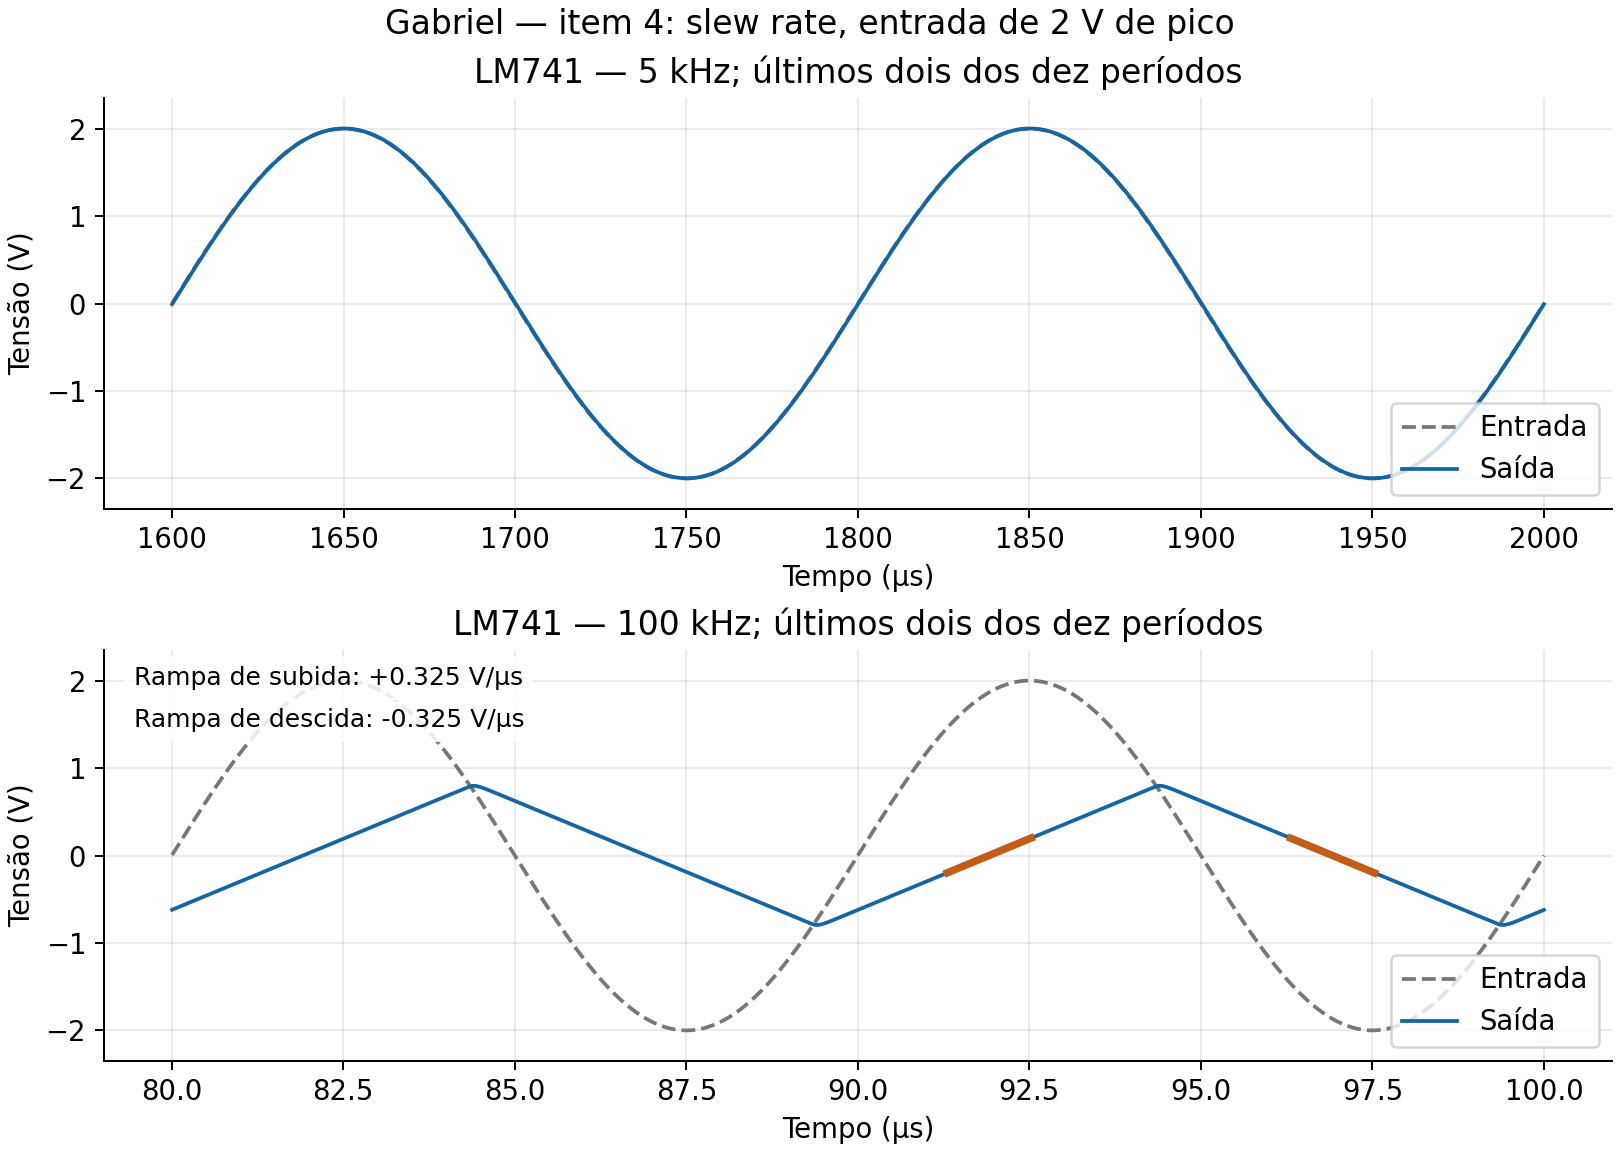
\includegraphics[width=\linewidth]{gabriel/item_4_grafico.png}
\caption{Gabriel, item\_4: entrada e saída do LM741 em \(5\) e \(100\,\text{kHz}\),
com \(V_p=2\,\text{V}\). São exibidos os dois últimos períodos de cada simulação;
os trechos em laranja foram usados para ajustar as inclinações das rampas.}
\label{fig:gabriel-item4-grafico}
\end{figure}

\begin{figure}[H]
\centering
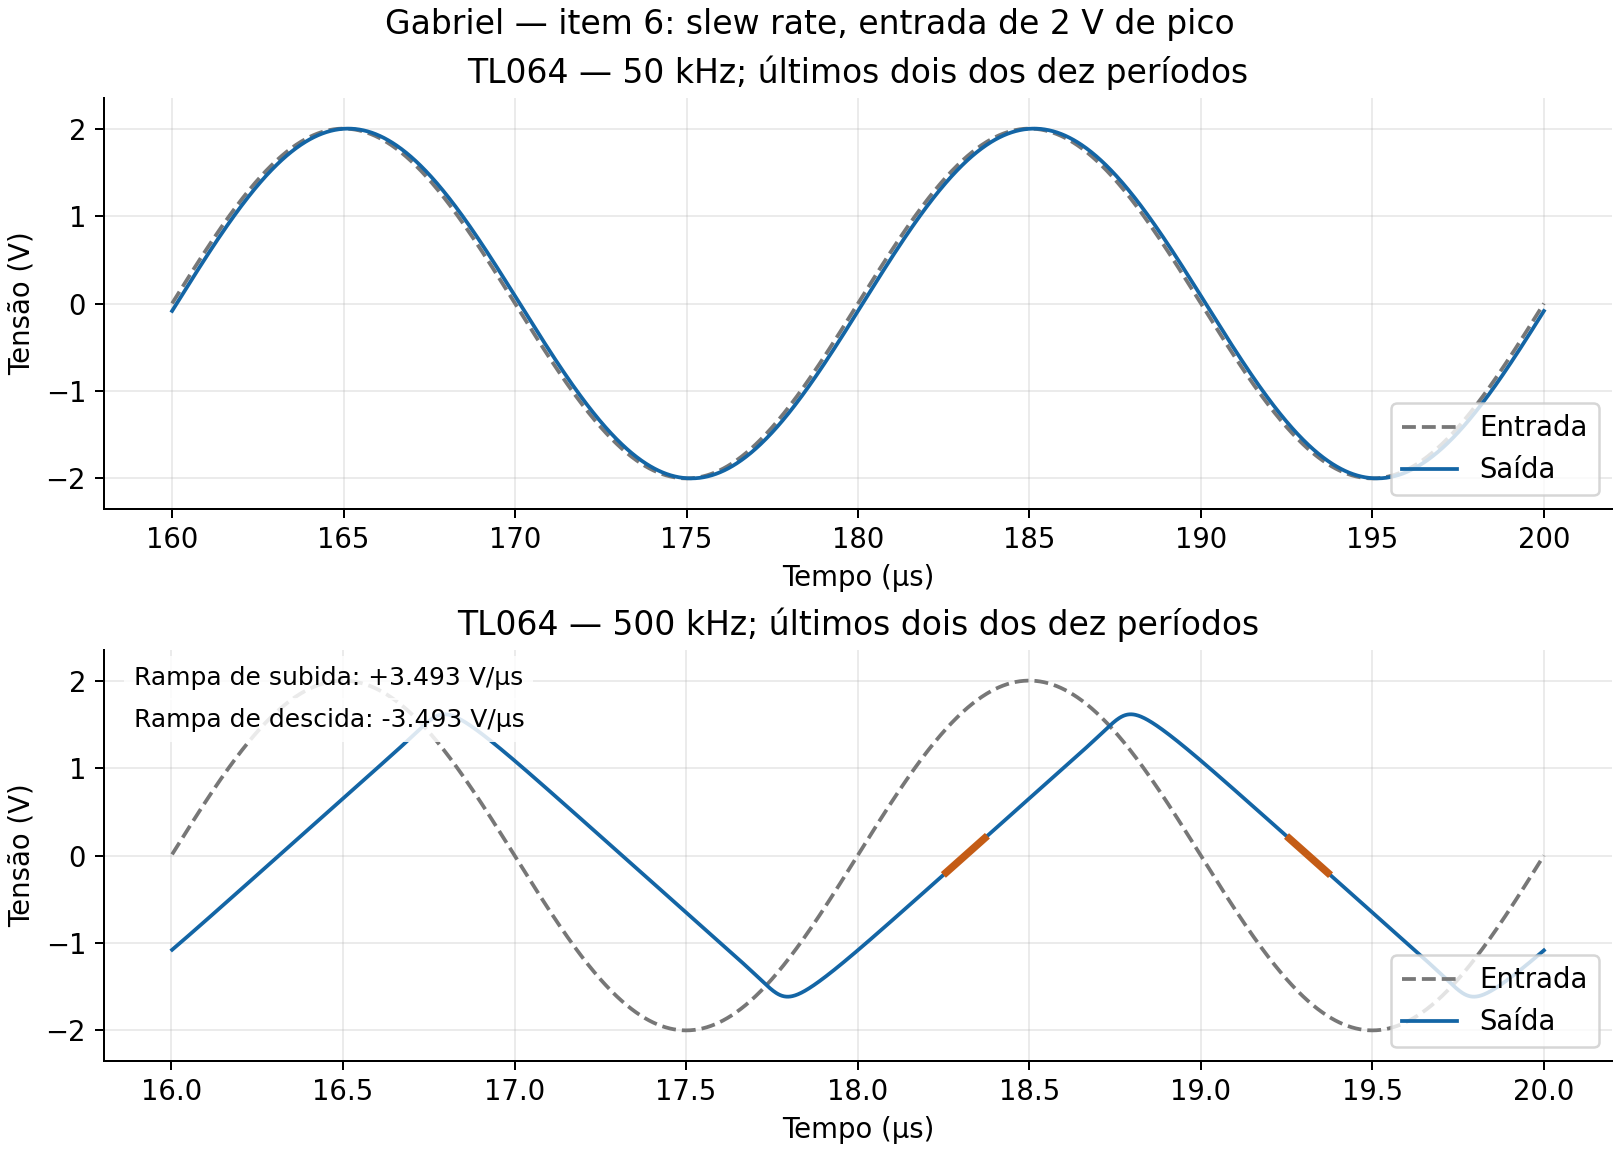
\includegraphics[width=\linewidth]{gabriel/item_6_grafico.png}
\caption{Gabriel, item\_6: entrada e saída do TL064 em \(50\) e \(500\,\text{kHz}\),
com \(V_p=2\,\text{V}\). As rampas destacadas permitem comparar as taxas de subida e descida.}
\label{fig:gabriel-item6-grafico}
\end{figure}

As inclinações foram obtidas por ajuste linear das amostras com
\(\lvert V_{out}\rvert<0{,}2\,\text{V}\) no último período da frequência alta,
separando subida e descida. No LM741, os intervalos foram
\(91{,}305\)--\(92{,}525\,\mu\text{s}\) e
\(96{,}311\)--\(97{,}531\,\mu\text{s}\), com taxas de
\(+0{,}3252\) e \(-0{,}3252\,\text{V}/\mu\text{s}\).
No TL064, foram \(18{,}258\)--\(18{,}370\,\mu\text{s}\) e
\(19{,}258\)--\(19{,}370\,\mu\text{s}\), com
\(+3{,}4931\) e \(-3{,}4927\,\text{V}/\mu\text{s}\).

Com \(V_p=2\,\text{V}\), os limites calculados com os típicos de datasheet são
\(39{,}79\,\text{kHz}\) para o LM741 e \(278{,}52\,\text{kHz}\) para o TL064.
Com as rampas simuladas, os limites são \(25{,}88\,\text{kHz}\) e
\(277{,}97\,\text{kHz}\), respectivamente. O LM741 simulado fica cerca de
\(35\%\) abaixo do típico de slew rate, enquanto o TL064 fica a menos de \(1\%\).
A razão entre as taxas simuladas é aproximadamente \(10{,}74\).
Esses resultados pertencem ao ensaio de Gabriel; as amplitudes e frequências dos
ensaios de Ana são diferentes, e seus valores foram mantidos na tabela anterior.

\subsection{Tensão de offset (Seção 3.3)}

\begin{center}\small
\setlength{\tabcolsep}{4pt}
\begin{tabular}{@{}lrrl@{}}
\toprule
\textbf{Medida} & \textbf{Previsto (sim.)} & \textbf{Datasheet} & \textbf{Medido} \\
\midrule
LM741 nº1, \(V_o\) (fio no pino~3) & \(108{,}189\,\text{mV}\) & até \({\approx}500\,\text{mV}\) &
  \(15{,}306\,\text{mV}\) \\
LM741 nº1, \(V_{os}\) (\(G{=}98{,}058\) medido) & \({\approx}1{,}1\,\text{mV}\) & 1 mV típico, 5 mV máx. & \(0{,}1561\,\text{mV}\) \\
LM741 nº2, \(V_o\) (fio no pino~3) & \(108{,}189\,\text{mV}\) & até \({\approx}500\,\text{mV}\) &
  \(16{,}339\,\text{mV}\) \\
LM741 nº2, \(V_{os}\) (\(G{=}98{,}058\) medido) & \({\approx}1{,}1\,\text{mV}\) & 1 mV típico, 5 mV máx. & \(0{,}1666\,\text{mV}\) \\
\bottomrule
\end{tabular}
\end{center}

As duas leituras precisaram de um capacitor de \(100\,\text{nF}\) da saída ao terra para parar de
oscilar no último dígito do multímetro. Essa observação é compatível com redução de ruído
na leitura, mas não identifica isoladamente sua origem. Não há valor residual registrado
após ajuste por potenciômetro; a comparação de offset usa as leituras sem ajuste.

\textbf{Questão (onde \(V_{os}\) cai na faixa do datasheet, e com o outro amplificador?).} As
duas peças mediram \(V_{os}\) uma ordem de grandeza \emph{abaixo} do típico de datasheet
(\(0{,}156\)--\(0{,}167\,\text{mV}\) contra \(1\,\text{mV}\) típico), e confortavelmente dentro do
máximo (\(5\,\text{mV}\)). A troca de amplificador (segundo LM741, mesma montagem) deu um valor
muito próximo do primeiro (\(16{,}339\) contra \(15{,}306\,\text{mV}\), \(6{,}8\%\) de diferença
entre as duas peças) — consistente com o datasheet descrever um valor típico de uma distribuição
de peças, não uma garantia individual, sem implicar que as duas peças tenham exatamente os mesmos parâmetros.

\subsection{Corrente de polarização (Seção 3.4)}

\begin{center}\small
\setlength{\tabcolsep}{4pt}
\begin{tabular}{@{}lrrl@{}}
\toprule
\textbf{Medida} & \textbf{Previsto (sim.)} & \textbf{Datasheet} & \textbf{Medido} \\
\midrule
LM741, \(V_o\) com \(R_s{=}98{,}9\,\text{k}\Omega\) & \(-452{,}581\,\text{mV}\) & — & \(-472{,}332\,\text{mV}\) \\
LM741, \(\Delta V_o\) & \(-560{,}770\,\text{mV}\) & \({\approx}{-}776\,\text{mV}\) (típico) & \(-487{,}638\,\text{mV}\) \\
LM741, \(I_b\) (\(G,R_s\) medidos) & \({\approx}58\,\text{nA}\) & 80 nA típico, 500 nA máx. & \({\approx}50{,}3\,\text{nA}\) \\
TL064, \(V_o\) (fio) & \(2{,}62514\,\text{mV}\) & — & \(2{,}792\,\text{mV}\) \\
TL064, \(V_o\) com \(R_s\) & \(2{,}62514\,\text{mV}\) & — & \(2{,}632\,\text{mV}\) \\
TL064, \(\Delta V_o\) & — & — & \(-0{,}160\,\text{mV}\) \\
TL064, \(I_b\) (\(G,R_s\) medidos) & \({\approx}0\) & dezenas de pA & \({\approx}16{,}5\,\text{pA}\) \\
\bottomrule
\end{tabular}
\end{center}

O registro experimental desta seção é constituído pelas leituras de multímetro
apresentadas na Figura~\ref{fig:bancada-34}.

\textbf{Questão (sentido da corrente, e o que aconteceu ao trocar de peça).} A saída
\textbf{desceu} nas duas peças quando \(R_s\) entrou (de \(+15{,}306\) para
\(-472{,}332\,\text{mV}\) no LM741; de \(2{,}792\) para \(2{,}632\,\text{mV}\) no TL064) — pela
Equação~\eqref{eq:bias}, \(\Delta V_o<0\) significa que a corrente na verdade entra no pino não
inversor, drenada da malha externa: o comportamento esperado de um par de entrada bipolar NPN
(LM741), que precisa de corrente de base fornecida externamente. O degrau do TL064
(\(0{,}160\,\text{mV}\)) é cerca de \(3050\times\) menor que o do LM741
(\(487{,}638\,\text{mV}\)) — \(I_b(\text{TL064}){\approx}16{,}5\,\text{pA}\) contra
\(I_b(\text{LM741}){\approx}50{,}3\,\text{nA}\) —, porque o TL064 tem entrada JFET, cujo terminal
de porta praticamente não drena corrente contínua, ao contrário da base bipolar do LM741.

\subsection{Resposta em frequência (Seção 3.5)}
\label{sec:freq-bancada}

As tabelas apresentam os pontos com frequência e amplitudes registradas. Os ganhos
foram calculados por \(V_{out,pp}/V_{in,pp}\). A classificação das formas de onda
acompanha os registros do ensaio.

\begin{center}\small
\setlength{\tabcolsep}{4pt}
\begin{tabular}{@{}lrrrrl@{}}
\toprule
\textbf{Ganho 11} & \textbf{Freq.} & \(V_{in}\) (Vpp) & \(V_{out}\) (Vpp) & \(G\) & \textbf{Onda} \\
\midrule
Referência & \(100{,}0\,\text{Hz}\) & \(181{,}03\,\text{mV}\) & \(2{,}05\,\text{V}\) & \(11{,}32\) & senoide \\
& \(10{,}0\,\text{kHz}\) & \(180{,}8\,\text{mV}\) & \(2{,}03\,\text{V}\) & \(11{,}23\) & senoide \\
& \(40{,}0\,\text{kHz}\) & \(182{,}1\,\text{mV}\) & \(1{,}89\,\text{V}\) & \(10{,}38\) & senoide \\
& \(60{,}0\,\text{kHz}\) & \(182{,}67\,\text{mV}\) & \(1{,}58\,\text{V}\) & \(8{,}649\) & \emph{triangular} \\
& \(70{,}0\,\text{kHz}\) & \(182{,}6\,\text{mV}\) & \(1{,}64\,\text{V}\) & \(8{,}98\) & \emph{triangular} \\
Próximo de \(-3\,\text{dB}\) & \(\mathbf{91{,}00\,\text{kHz}}\) & \(182{,}9\,\text{mV}\) & \(1{,}48\,\text{V}\) & \(\mathbf{8{,}09}\) & \emph{triangular} \\
& \(110\,\text{kHz}\) & \(182{,}1\,\text{mV}\) & \(1{,}32\,\text{V}\) & \(7{,}25\) & \emph{triangular} \\
& \(300\,\text{kHz}\) & \(181{,}0\,\text{mV}\) & \(0{,}59\,\text{V}\) & \(3{,}26\) & \emph{triangular} \\
\bottomrule
\end{tabular}
\end{center}

\begin{center}\small
\setlength{\tabcolsep}{4pt}
\begin{tabular}{@{}lrrrrl@{}}
\toprule
\textbf{Ganho 101} & \textbf{Freq.} & \(V_{in}\) (Vpp) & \(V_{out}\) (Vpp) & \(G\) & \textbf{Onda} \\
\midrule
Referência & \(100{,}0\,\text{Hz}\) & \(19{,}83\,\text{mV}\) & \(1{,}95\,\text{V}\) & \(98{,}34\) & senoide \\
& \(2{,}0\,\text{kHz}\) & \(19{,}82\,\text{mV}\) & \(1{,}93\,\text{V}\) & \(97{,}4\) & senoide \\
& \(5{,}0\,\text{kHz}\) & \(19{,}89\,\text{mV}\) & \(1{,}86\,\text{V}\) & \(93{,}5\) & senoide \\
& \(9{,}9\,\text{kHz}\) & \(17{,}8\,\text{mV}^{*}\) & \(1{,}48\,\text{V}\) & \(83{,}15\) & senoide \\
& \(50{,}0\,\text{kHz}\) & \(19{,}72\,\text{mV}\) & \(0{,}57\,\text{V}\) & \(28{,}9\) & senoide \\
\bottomrule
\end{tabular}
\end{center}

{\small \(^{*}\)A entrada em \(9{,}9\,\text{kHz}\) foi de \(17{,}8\,\text{mV}_{pp}\),
abaixo dos aproximadamente \(19{,}8\,\text{mV}_{pp}\) dos demais pontos; o ganho usa a
amplitude efetivamente registrada nesse ponto.}

No ganho baixo, a referência de \(2{,}05\,\text{V}_{pp}\) corresponde a
\(1{,}025\,\text{V}\) de pico, enquanto o roteiro especifica \(0{,}2\,\text{V}\).
Em \(91\,\text{kHz}\), o ganho relativo é \(8{,}092/11{,}324=0{,}715\), próximo
de \(0{,}707\), porém com saída classificada como triangular. O produto
\(11{,}324\times91\,\text{kHz}=1{,}0305\,\text{MHz}\) é apenas um produto entre
ganho de referência e frequência observada; a distorção impede identificá-lo como
medida isolada do GBW.

No ganho alto, foi ajustado o modelo de um polo
\[
\frac{G(f)}{G_{ref}}=\frac{1}{\sqrt{1+(f/f_c)^2}},
\qquad G_{ref}=\frac{1{,}95}{0{,}01983}=98{,}336.
\]
O ajuste minimiza a soma dos quadrados dos resíduos de ganho normalizado nos quatro
pontos acima de \(100\,\text{Hz}\), com pesos iguais, e fornece
\(f_c\approx15{,}50\,\text{kHz}\). As estimativas individuais dos pontos de
\(2\), \(5\), \(9{,}9\) e \(50\,\text{kHz}\) são, respectivamente,
\(14{,}21\), \(15{,}37\), \(15{,}68\) e \(15{,}38\,\text{kHz}\).
O resultado é uma estimativa dependente do modelo, não uma leitura direta no corte;
o produto correspondente é \(G_{ref}f_c\approx1{,}524\,\text{MHz}\).
As razões adicionais de ganho \(0{,}790\) e \(0{,}702\), sem pares completos de
frequência e amplitudes, não foram usadas no ajuste.

\begin{figure}[H]
\centering
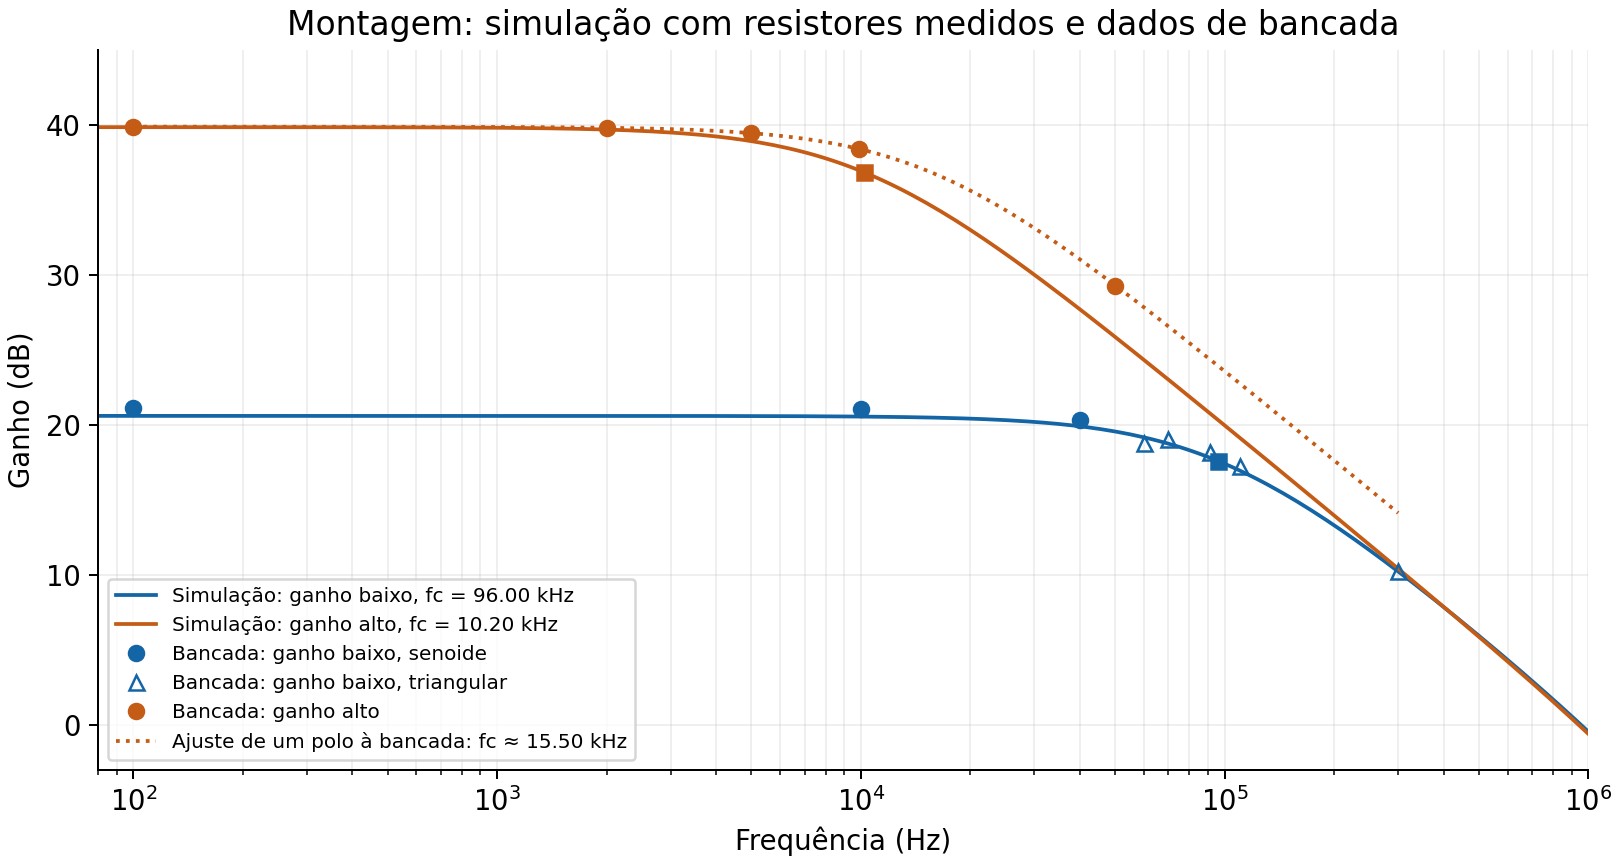
\includegraphics[width=\linewidth]{gabriel/montagem_frequencia.png}
\caption{Resposta em frequência: curvas contínuas da simulação com resistores medidos,
pontos de bancada e ajuste de um polo ao ganho alto (pontilhado). Os quadrados indicam
os cortes simulados; os triângulos vazados indicam medidas com saída triangular.
As curvas AC representam pequeno sinal e não modelam a distorção dos pontos triangulares.}
\label{fig:bancada-35-grafico}
\end{figure}

\textbf{Influência da amplitude.} A saída de menor amplitude no ganho baixo é necessária
porque sua banda passante é maior. Com o slew rate medido de
\(0{,}314\,\text{V}/\mu\text{s}\), uma senoide de \(1{,}025\,\text{V}\) de pico exige
mais que essa taxa acima de aproximadamente \(48{,}8\,\text{kHz}\); com
\(0{,}2\,\text{V}\), o limiar sobe para \(249{,}9\,\text{kHz}\), acima do corte
simulado de \(96\,\text{kHz}\). Isso explica a importância da amplitude prescrita
para medir a resposta linear. O aparecimento de ondas triangulares nos registros a
partir de \(60\,\text{kHz}\) é consistente com essa limitação. No ganho alto, o corte
é menor, permitindo usar saída de aproximadamente \(1\,\text{V}\) de pico com menor
influência de slew rate na vizinhança do corte.

A faixa registrada alcança \(300\,\text{kHz}\) no ganho baixo e \(50\,\text{kHz}\)
no alto. O conjunto completo contém oito pontos no primeiro e cinco no segundo;
a caracterização experimental não cobre uma década inteira acima dos cortes de referência.

\subsection{Slew rate (Seção 3.6)}

\begin{center}\small
\setlength{\tabcolsep}{4pt}
\begin{tabular}{@{}lrr@{}}
\toprule
\textbf{Grandeza} & \textbf{LM741} & \textbf{TL064} \\
\midrule
Frequência do registro triangular & \(39{,}7\,\text{kHz}\) & \(447{,}0\,\text{kHz}\) \\
\(\Delta V\), cursores & \(2{,}47\,\text{V}\) & \(2{,}74\,\text{V}\) \\
\(\Delta t\), cursores & \(7{,}860\,\mu\text{s}\) & \(0{,}796\,\mu\text{s}\) \\
\(SR\) medido & \(0{,}314\,\text{V}/\mu\text{s}\) & \(3{,}442\,\text{V}/\mu\text{s}\) \\
\(SR\) simulado na montagem & \(0{,}3252\,\text{V}/\mu\text{s}\) & \(3{,}4848\,\text{V}/\mu\text{s}\) \\
\(SR\) típico de datasheet & \(0{,}5\,\text{V}/\mu\text{s}\) & \(3{,}5\,\text{V}/\mu\text{s}\) \\
\(f_{max}\), com \(SR\) medido & \(25{,}0\,\text{kHz}\) & \(273{,}9\,\text{kHz}\) \\
\(f_{max}\), com típico de datasheet & \(39{,}79\,\text{kHz}\) & \(278{,}52\,\text{kHz}\) \\
\bottomrule
\end{tabular}
\end{center}

As inclinações experimentais são as razões \(\Delta V/\Delta t\) das capturas da
Seção~\ref{sec:bancada}. Comparadas à simulação nas mesmas frequências e amplitude,
ficam aproximadamente \(3{,}5\%\) abaixo no LM741 e \(1{,}2\%\) abaixo no TL064.
O LM741 apresenta maior diferença em relação ao típico de datasheet; o TL064 fica
próximo desse valor. O macromodelo descreve essas rampas mais de perto que o valor
típico do LM741, sem representar necessariamente todos os parâmetros de cada peça.

Com \(V_p=2\,\text{V}\), os limites calculados pela Equação~\eqref{eq:slew-fmax}
com os slew rates medidos são \(25{,}0\) e \(273{,}9\,\text{kHz}\).
As capturas triangulares foram obtidas acima desses limites, em frequências
aproximadamente \(1{,}6\) vez maiores, coerentemente com o aumento da distorção.
A razão entre os slew rates medidos é \(3{,}442/0{,}314=10{,}96\), comparada a
\(10{,}71\) na simulação da montagem e \(7\) entre os típicos de datasheet.

A frequência de corte \emph{linear de pequeno sinal} não depende da amplitude.
A frequência aparente de atenuação de uma medida com distorção pode depender dela,
pois o limiar de slew rate varia com \(1/V_p\). Essa distinção explica por que a
varredura do ganho baixo não permite separar os dois efeitos por amplitude apenas.

\section{Discussão}
\label{sec:discussao}

\textbf{Projeto e componentes medidos.} Os projetos individuais realizam os ganhos
especificados para cada matrícula. Na montagem, os resistores medidos levam a ganhos
calculados de \(10{,}689\) e \(98{,}058\), próximos dos valores AC simulados de
\(10{,}689\) e \(98{,}013\). As diferenças de ganho nominal decorrentes dos resistores
são distintas das diferenças entre o modelo do amplificador e as peças de bancada.

\textbf{Offset e polarização.} O LM741 simulado com resistores medidos fornece
\(V_o=108{,}189\,\text{mV}\), enquanto os exemplares de bancada apresentam
\(15{,}306\) e \(16{,}339\,\text{mV}\). O offset é dependente do exemplar, e o modelo
não foi ajustado às peças utilizadas. Por isso, a comparação de corrente é mais
informativa pela diferença entre saídas do que pela saída com \(R_s\) isoladamente:
\(\lvert\Delta V_o\rvert\) é \(560{,}770\,\text{mV}\) na simulação e
\(487{,}638\,\text{mV}\) na bancada. A corrente calculada, \(50{,}3\,\text{nA}\),
fica cerca de \(13\%\) abaixo dos \(57{,}824\,\text{nA}\) simulados.
No TL064, o pequeno degrau de \(0{,}160\,\text{mV}\) corresponde a
\(16{,}5\,\text{pA}\), efeito que o modelo fornecido não reproduz em DC.
A razão experimental entre as correntes é aproximadamente \(3{,}05\times10^3\).

\textbf{Resposta em frequência.} Na simulação, os produtos ganho-corte de
\(1{,}0262\) e \(0{,}9997\,\text{MHz}\) diferem em cerca de \(2{,}6\%\), mostrando
a constância aproximada esperada. Na bancada, o estágio baixo opera com amplitude
acima da prescrita e apresenta saída triangular; seu produto de \(1{,}0305\,\text{MHz}\)
não constitui validação independente do GBW, apesar da proximidade numérica.
No estágio alto, o ajuste aos pontos completos fornece \(15{,}50\,\text{kHz}\),
contra \(10{,}20\,\text{kHz}\) na simulação. O produto estimado de
\(1{,}524\,\text{MHz}\) é aproximadamente \(52\%\) maior que o simulado.
A variação dos resistores já foi incluída e não explica essa diferença. Variação
entre o exemplar e o modelo, incertezas de amplitude e condições de montagem são
hipóteses compatíveis; os registros não permitem atribuir uma causa única.
Não foi construída uma incerteza quantitativa, pois não há série de repetições nem
propagação das especificações instrumentais para estes pontos.

\textbf{Slew rate.} As rampas medidas ficam próximas das simuladas nas mesmas
condições, com desvios menores que \(4\%\), e mostram o TL064 aproximadamente onze
vezes mais rápido que o LM741. As frequências das capturas triangulares superam os
limites calculados para início da limitação, como esperado para uma distorção já visível.

\textbf{Alcance experimental.} A ausência de leitura residual após o ajuste de offset
limita a análise às peças sem compensação. O registro de polarização contém as leituras
de multímetro, sem fotografias das respectivas montagens. A documentação não confirma
o desacoplamento de cada alimentação, e a varredura do ganho alto tem cinco pontos
completos. Essas condições delimitam o alcance das comparações experimentais.

\section{Conclusão}
\label{sec:conclusao}

Os ensaios caracterizaram offset, polarização, resposta em frequência e slew rate,
complementados por simulações dos projetos individuais e da montagem com resistores medidos.
Os dois LM741 apresentaram offsets equivalentes de \(0{,}156\) e \(0{,}167\,\text{mV}\),
enquanto a comparação de polarização indicou corrente aproximadamente três mil vezes
menor no TL064. O modelo do LM741 forneceu corrente da mesma ordem da experimental;
o do TL064 não reproduziu o pequeno valor DC obtido na bancada.

A simulação confirmou a relação aproximada entre ganho e banda, com cortes de
\(96{,}00\) e \(10{,}20\,\text{kHz}\) na montagem. Na bancada, a distorção do ganho
baixo impede isolar seu corte linear; no ganho alto, o ajuste de um polo estimou
\(15{,}50\,\text{kHz}\), com diferença expressiva em relação ao modelo.
Os slew rates de \(0{,}314\) e \(3{,}442\,\text{V}/\mu\text{s}\) ficaram próximos
dos simulados e evidenciaram a resposta mais rápida do TL064. A comparação mostra
que largura de banda e slew rate exigem condições de ensaio diferentes: a primeira
é uma propriedade de pequeno sinal, enquanto a limitação pelo segundo depende da taxa
de variação exigida pela combinação de amplitude e frequência.

\section{Referências}

\begin{referencias}
\item SEDRA, A.~S.; SMITH, K.~C. \emph{Microeletrônica}. 5.~ed. São Paulo: Pearson
      Prentice Hall, 2007.
\item BOYLESTAD, R.~L.; NASHELSKY, L. \emph{Dispositivos Eletrônicos e Teoria de
      Circuitos}. 11.~ed. São Paulo: Pearson Education do Brasil, 2013.
\item Texas Instruments. \emph{LM741 Operational Amplifier}. SNOSC25D, 2015.
\href{https://www.ti.com/lit/ds/symlink/lm741.pdf}{Datasheet do LM741}.
\item Texas Instruments. \emph{TL06xx Low-Power JFET-Input Operational Amplifiers}.
\href{https://www.ti.com/lit/ds/symlink/tl064.pdf}{Datasheet da família TL06xx}.
\end{referencias}

\end{document}
